% This is LLNCS.DEM the demonstration file of
% the LaTeX macro package from Springer-Verlag
% for Lecture Notes in Computer Science,
% version 2.3 for LaTeX2e
\documentclass{llncs}

% PACKAGES
\usepackage{mathtools}
\usepackage{float}
\usepackage{url}
\usepackage{graphicx}
\usepackage{amssymb}
\usepackage{makeidx}  % allows for indexgeneration
\usepackage[style=math, tight]{k}
\usepackage{listings,xcolor}
\usepackage{inconsolata}
\usepackage[position=top]{subfig}
\usepackage{pgfplots}


\floatstyle{plain}
\restylefloat{figure}

\definecolor{dkred}{rgb}{.6,0,0}
\definecolor{dkgreen}{rgb}{0,.5,0}
\definecolor{dkblue}{rgb}{0,0,.6}
\definecolor{dkyellow}{cmyk}{0,0,.8,.3}



\lstset{
  language        = php,
  morekeywords = [1]{class, private, public, protected, static, extends, function,parent,self,new,global,is_float,var_dump,boolean,integer,float,string,object,},
  basicstyle      = \footnotesize\ttfamily,
  keywordstyle    = \color{dkblue},
  stringstyle     = \color{dkred},
  identifierstyle = \color{dkgreen},
  commentstyle    = \color{gray},
  emph            =[1]{php},
  emphstyle       =[1]\color{black},
  emph            =[2]{if,and,or,else},
  emphstyle       =[2]\color{dkyellow},
  literate = {??}{{\#}}1,}


\newcommand{\etal}{\emph{et al.}}
\newcommand{\HOLE}{$\Box$}
\newcommand{\kfrac}[2]{$\frac{\big #1}{\big #2}$}

\newcommand{\kc}[1]{\texttt{\small #1}}
\let\cc\lstinline


% MACROS 

\newif\iflong\longtrue
\longfalse
\newif\ifdraft\drafttrue
\draftfalse

\newcommand{\kphp}{${\K\text{PHP}}$}
%\newcommand{\kphp}{$\K_{\text{PHP}}$}
\newcommand{\website}{\url{http://phpsemantics.org}}
%\newcommand{\etal}{\emph{et al.}}

% comments

\newcommand{\displaycomment}[1]{\marginpar{\raggedright\scriptsize{#1}}} % on margin
% \newcommand{\displaycomment}[1]{{#1}} % inline
\newcommand\hl[1]{{\color{dkred} #1}}

%\newcommand{\displaycomment}[1]{}
%\newcommand\hl[1]{#1}%

\newcommand{\todonote}[2]{\displaycomment{{\color{dkred}{\bf todo (#1): }#2}}}
\newcommand{\xremark}[2]{\displaycomment{{{\color{dkgreen}(#1: #2)}}}}

\ifdraft
\newcommand{\SM}[1]{\todonote{SM}{#1}}
\newcommand{\sm}[1]{\xremark{SM}{#1}}
\newcommand{\DF}[1]{\todonote{DF}{#1}}
\newcommand{\df}[1]{\xremark{DF}{#1}}
\else
\newcommand{\SM}[1]{}
\newcommand{\sm}[1]{}
\newcommand{\DF}[1]{}
\newcommand{\df}[1]{}
\fi

\def\myparagraph#1{\vspace{0.3em}\noindent{\textbf{#1.}}}
\newcommand{\stitle}{\myparagraph}





% Including artefact commands
% Commands for one-page artifact description appendices in lncs volumes
% Written by Camil Demetrescu and Erik Ernst
% April 8, 2014

% ARTIFACT: This entire file should be used as-is; it defines standard
% headings to be included in the artifact description, and it will be 'input'
% into the file artifact.tex such that you can use the environments defined
% below

\newcommand{\artifactauthors}[1]{{\paragraph{\bf Authors of the artifact.}#1}}
\newenvironment{summary}{\paragraph{\bf Summary.}}{}
\newenvironment{content}{\paragraph{\bf Content.}}{}
\newenvironment{getting}{\paragraph{\bf Getting the artifact.} }{}
\newenvironment{platforms}{\paragraph{\bf Tested platforms.}}{}
\newcommand{\license}[1]{{\paragraph{\bf License.}#1}}
\newcommand{\mdsum}[1]{{\paragraph{\bf MD5 sum of the artifact.}#1}}
\newcommand{\artifactsize}[1]{{\paragraph{\bf Size of the artifact.}#1}}
\newcommand{\AEBadge}{%
  \raisebox{-9mm}[-15mm][0pt]{%
    \hspace{-39mm}%
    \includegraphics[width=15mm]{aec-badge-ecoop}%
    \hspace{22.5mm}}}


\begin{document}

\frontmatter          % for the preliminaries

% TITLE
\title{An executable formal semantics of PHP\iflong \thanks{This is the extended version (revised \today) of the homonymous paper to appear at ECOOP 2014.}\fi}

%\ifdraft
\author{Daniele Filaretti \and Sergio Maffeis}
%\authorrunning{D. Filaretti and S. Maffeis}   % abbreviated author list (for running head)
%%%% list of authors for the TOC (use if author list has to be modified)
%\tocauthor{Daniele Filaretti, Sergio Maffeis}
\institute{
	Department of Computing, Imperial College London\\ \email{\{d.filaretti11,sergio.maffeis\}@imperial.ac.uk}
}
%\fi
\maketitle          



\begin{abstract}
\iflong\else \AEBadge{}\fi
PHP is among the most used languages for server-side scripting. Although substantial effort has been spent on the problem of automatically analysing PHP code, vulnerabilities remain pervasive in web applications, and analysis tools do not provide any formal guarantees of soundness or coverage.
This is partly due to the lack of a precise specification of the language, which is highly dynamic and often exhibits subtle behaviour. 

We present the first formal semantics for a substantial core of PHP, based on the official documentation and experiments with the Zend reference implementation. Our semantics is executable, and is validated by testing it against the Zend test suite.
%
We define the semantics of PHP in a term-rewriting framework which supports LTL model checking and symbolic execution. As a demonstration, we extend LTL with predicates for the verification of PHP programs, and analyse two common PHP functions.

\end{abstract}




% OLD ABSTRACT
%
%PHP is the most common language for server-side web programming. Although substantial effort has already been spent on the problem of automatically analyzing PHP code, vulnerabilities remain pervasive in deployed web applications. This is in part due to the dynamic nature of the language, its sometimes subtle behaviour, and the lack of a precise specification. Moreover, the available analysis tools do not provide any formal guarantees of soundness or coverage.
%
%As a step towards rigorous, automated formal analysis of PHP applications, this paper presents the first formal semantics for a substantial core of the PHP programming language, based on the official documentation as well as experiments with the reference implementation. Our semantics is executable, and can be validated by testing against common PHP test suites. 
%%
%We define our semantics in a term-rewriting framework for reasoning about programming languages, which provides support for LTL model checking, and symbolic execution. We extend LTL with predicates for the verification of PHP programs, and we analyze non-trivial properties of two pervasive, third-party PHP functions.
%%
%\sm{last sentence may be too strong at the moment, need to revise this}
%






% -------------------------------
% --- INTRODUCTION ---
% -------------------------------
\section{Introduction}\label{sec:intro}

% PHP is popular
PHP is one of the most popular languages for server-side scripting, used by 
amateur web developers as well as billion-dollar companies such as Google, Facebook and Yahoo!.
It is used for developing complex programs, enabling all sort of sensitive activities such as online banking, social networking, and cloud computing. 
%
% Dynamic features lead to bugs
Despite the flexibility and ease of use of PHP, its dynamic features 
(shared by similar scripting languages) make it easy to introduce errors in programs,
potentially opening security holes leading to the leakage of sensitive data and other forms of compromise.

% Web attacks
%Although the nature of many web attacks (XSS, CSRF, SQL injection, etc.) is now well understood, and despite a large amount of academic literature on the subject, most of the web applications out there still contain vulnerabilities, and PHP is one of the major culprits. Indeed, the problem seems to be growing with the dimension and complexity of the applications themselves. 

Many web applications have reached a level of complexity for which testing, code reviews and human inspection are no longer sufficient quality-assurance guarantees.
%
%The problem of automatically detecting and, where possible, fixing vulnerabilities in web applications remains open.
%
% Static analysis
Tools that employ static analysis techniques~\cite{Cousot1977,Pierce2002,Hjelseth2010} are needed in order explore all possible execution paths through an application, and guarantee the absence of undesirable behaviours. 
However, due to classic computability results, this goal can be accomplished only by applying a certain degree of abstraction, with consequent loss of precision (i.e. introducing false positives).
%
To make sure that an analysis captures the properties of interest, and to navigate the trade-offs between efficiency and precision, it is necessary to base the design and, we add, the development, of static analysis tools on a firm understanding of the language to be analysed.

The main contribution of this paper is to present \kphp, the first formal (and executable) semantics of PHP, which can serve as a basis to define program analyses and semantics-based verification tools (Section~\ref{sec:kphp}). 

% Langauge specifications
Some programming languages, such as Standard ML~\cite{Milner1997}, already come with a formal specification.
Others, such as C~\cite{New2012} and JavaScript~\cite{Ecma2009} are specified in English prose with varying degrees of rigour and precision, and have recently been formalised~\cite{Norrish1998,Maffeis2008,Blazy2009,Guha2010,Ellison2012,Bodin}. 
%
PHP is only implicitly defined by its \emph{de facto} reference implementation (the Zend Engine~\cite{zend}), and the (informal) PHP reference manual~\cite{PHP-docs}.
%
Due to the lack of a document providing a precise specification of PHP, defining its formal semantics is particularly challenging. We have to rely on the approximate information available online, and a substantial amount of testing against the reference language implementation. 
%
We do not to base our semantics on the source code of the Zend Engine in order to avoid bias towards inessential implementation choices.
%
In defining our semantics, we identify several cases where the behaviour of PHP is complicated and unexpected. 
Some of these examples are known to PHP programmers, and have contributed to driving our design. 
Other examples are new, and were discovered by us as a consequence of semantic modelling (Section~\ref{sec:php}).
%
Although useful to get introduced to each language construct, the online PHP language reference~\cite{PHP-docs} is not precise enough to serve as a basis for a formal semantics. Quite the opposite, we hope that our formal semantics may serve as a basis to create a precise, English prose specification of PHP in the style of the ECMA specification of JavaScript~\cite{Ecma2009}. 


% Semanitcs in K
We write our semantics in \K~\cite{K-web,Rosu2010}, a framework for defining programming languages on top of the Maude~\cite{Clavel2002} term-rewriting tool.  
%
A language semantics as expressed in \K\ has a rigorous meaning as a term rewriting system, and is suitable for formal reasoning and automated proofs. Moreover, it is directly executable, enabling a tight design-test loop which is crucial for the test-driven semantics development needed in the case of PHP. 
%
%% LONG:
%By contrast, the reference JavaScript interpreter associated to JSCert is the result of the automatic extraction of OCAML code from a fix-point Coq definition that needs to be kept manually in sync ...
% \sm{we could criticise: jscert, as in our case sem IS interp, so incompletness does not matter.}
%
% Need to test a semantics
Extensive testing using official test suites is becoming ``best practice'' to validate executable semantics of programming languages~\cite{Guha2010,Ellison2012,Bodin}.
%
We validate \kphp\ by automated testing against the Zend PHP test suite~\cite{zendtest} (Section~\ref{sec:testing}), and we design additional PHP tests in order to cover all of the semantic rules, including those not exercised by~\cite{zendtest}.

The main goal of our semantics is to provide a formal model of PHP upon which semantics-based verification tools (such as abstract interpreters, type systems and taint-checkers) can be built. Developing such tools goes beyond the scope of this paper. 
%
However, we are able to begin demonstrating the practical relevance of \kphp\ by using it for program verification. In particular, the \K\ framework exposes Maude's explicit-state Linear Temporal Logic (LTL) model checking to the semantics~\cite{Ellison2012}, and supports symbolic execution for any language definition~\cite{Arusoaie2012b}.
We define an extension of LTL with predicates to express interesting temporal properties of PHP programs, and verify two representative PHP functions from \texttt{phpMyAdmin}~\cite{phpMyAdminWeb} and the PHP documentation~\cite{pbkdf2Web} (Section~\ref{sec:applications}).


\iflong The \else An extended version of this paper, together with the \fi latest version of the semantics, and all the \kphp\ development (including \kphp\ interpreter, tests and verification examples) is available on \website.



















% -------------------------------
% --- A PHP Primer
% -------------------------------

\sm{we do not mention ``taint mode" anywhere!}

\section{A PHP Primer}\label{sec:php}
%
In this Section, we give a brief introduction to the PHP language and its usage, and present examples of some challenging and surprising features of the language.
\footnote{All the examples are reproducible by pasting the code in the PHP Zend Interpreter (version 5.3.26 or similar) available in most OSX or Linux distributions. The symbol \cc{>} precedes the shell output. For readability, here we re-format the output of \cc{var_dump}.}
%
Some of these examples are known to PHP programmers, and have contributed to driving the design of our semantics. Others are new, and were discovered by us, as a consequence of semantic modelling.







\iflong \subsection{Hello World Wide Web}\else
\stitle{Hello World Wide Web} \fi
%
PHP scripts are typically run by web servers. Typing a URL such as \iflong
\[\texttt{http://example.com/hello.php?name=xyz}\]
\else\texttt{http://example.com/hello.php?name=xyz}\fi in a browser may cause the responding server to invoke PHP on the file \texttt{hello.php} listed below:
%
\begin{lstlisting}
<? echo "<HTML><Body>Hello ".$_GET["name"]."!</Body></HTML>"; ?>
\end{lstlisting}
%
This minimal example illustrates the typical behaviour of a PHP script. It receives inputs from the web and it responds by generating an HTML page depending on such inputs. The predefined \cc{$_GET} array is in fact populated from the parameters of the HTTP request, and \cc{echo} is a simple output command that in shell mode prints to standard output but that in server mode generates the body of the HTTP response message.
%
In this paper, we focus on PHP as a programming language, and leave the important topic of formalisation of the server execution model to future work.











\subsection{PHP: a Closer Look}\label{sec:closerlook}

%We now describe some features of PHP which, despite being part of the core language, may be unfamiliar to programmers used to %different languages, or are challenging to represent in an operational semantics. 


We now describe some features of the core PHP language which may be unfamiliar to programmers used to different languages, challenging to represent in an operational semantics, or both. 

%We now describe some features of the core PHP language which are challenging to model in an operational semantics. 
%Some of these examples may be unfamiliar to programmers used to different languages. 




\stitle{Aliasing and references}
%
PHP supports variable aliasing via the \emph{assignment by reference} construct. This mechanism provides a means of accessing the same variable content by different names. 
%
\begin{lstlisting}
$x = 0;  
$y = &$x; 	// $x and $y are now aliased
$y = "Hello!";
echo $x; 	// prints "Hello!"
\end{lstlisting}
%
Aliasing can be useful for example to write functions that operate on parameters containing large data structures, avoiding the overhead of copying the data structure inside the local scope of the function.
%
On the other hand, aliasing is notoriously difficult to analyse statically.
%
PHP references are different from pointers (as in C) in that neither address-arithmetic nor access to arbitrary memory is allowed. For example, the following code would be rejected:
\begin{lstlisting}
$x = (&$x + 1);	// causes a parse error
\end{lstlisting}




\stitle{Braced and variable variables} 
%
The official PHP documentation gives the following description for \emph{variable variables}: ``A variable variable takes the value of a variable and treats that as the name of a variable''. Here is an example:
\begin{lstlisting}
$x = "y";  
$y = "Hello!";
echo $$x; 		// prints "Hello!"
\end{lstlisting}
%
Hence, in a PHP semantics, variable names should be modelled as a set of string-indexed constructors, rather than as a set of unforgeable identifiers.  

Variable variables are useful for example to simulate higher-order behaviour by passing functions \emph{by name}.
%
On the other hand, they hinder static analyses, because it is not possible in general to determine statically the set of variables used by a PHP script.
%
\sm{LONG: here we could say that HACK forbids them exactly for that reason}
%
A similar argument applies to braced variables, a syntax to turn the result of an arbitrary expression into an identifier, as for example in
\begin{lstlisting}
${"x"} = "y";  		// defines variable $x
$z -> {"x".$x};		// access field xy of object $z
\end{lstlisting}





\stitle{Type juggling}
%
Each PHP value has a type (\cc{boolean,integer},...). Automatic type conversions are performed when operators are passed operands of the incorrect type. For example, non-empty strings are translated to the boolean \cc{true}, and booleans \cc{true} and \cc{false} are converted respectively to the integers \cc{1} and \cc{0}.
%
\begin{lstlisting}
if ("false") echo true + false; else echo "false"; // prints "1"
\end{lstlisting}
%
Some type conversions need to be defined explicitly. For example, an object can be converted to a string by defining the \emph{magic method} \cc{__toString}. If such method is undefined, the attempted conversion triggers an exception.

Type juggling makes it easier to write code that does not get stuck, but also increases the probability that such code will not behave as expected. 
%
For example, although the conversion of objects to numbers is undefined according to the online documentation, the Zend engine converts objects to the integer \cc{1} (our semantics mimics this behaviour, and issues an additional warning). 




\stitle{Arrays}
%
Arrays in PHP are essentially \emph{ordered} maps from \cc{integer} or \cc{string} \emph{keys} to language values. If a value of a different type is given as a key, type juggling will try to convert it to an \cc{integer}.
\begin{lstlisting}
$x = array("foo" => "bar",4.5 => "baz"); 
\end{lstlisting}
The array \cc{$x} above maps \cc{"foo"} to \cc{"bar"} and \cc{4} to \cc{"baz"}. Note how the \cc{float} value \cc{4.5} was automatically converted to the \cc{integer} value \cc{4}.\footnote{Although we model array key conversions in our semantics, we do not give full details about them here. The interested reader can try evaluating this: \cc{$x = array( 1=>"foo", "2"=>"wow", 3.5=>"doh", "4.5"=>"omg",  NULL=>"lol" );}.}
%
Array elements can be accessed via standard square-bracket notation, and it is also possible to assign an element to an array without specifying a key. 
\begin{lstlisting}
$x[] = "default"	// use default key 5
$echo x[5] 		// prints "default"
\end{lstlisting}
In this case, a default key (the greatest integer key already defined, plus one) is used.
Arrays contain an internal pointer to the \emph{current} element (the first by default), which can be manipulated using functions \cc{current} \cc{next}, \cc{each} and \cc{reset}:
\begin{lstlisting}
echo current($x);	// prints "bar"
next($x);		// advances the pointer
echo current($x);	// prints "baz"
\end{lstlisting}


\stitle{Objects}
%
From a semantic standpoint, PHP objects can be seen as string-indexed arrays with additional visibility attributes (\cc{public}, \cc{protected} or \cc{static}), and with methods inherited by their defining class. 
Just like arrays, (\cc{stdClass}) objects can be initialised ``on the fly'':
\begin{lstlisting}
$obj -> x = 0;
var_dump($obj);
> object(stdClass)??1 (1) { ["x"]=> int(0) }
\end{lstlisting}
%
Access to an array element is always granted, whereas access to an object property is regulated by the visibility attribute, and depends on the context whence the property is being accessed.
%
Inheritance is class-based. Consider the following example from the Zend test suite~\cite{zendtest}:\\[7pt]
\hspace{-10pt}\begin{tabular}{ll|ll}
\begin{lstlisting}
class par {
  private $id = "foo";
  function displayMe() {
    echo $this -> id; }}
\end{lstlisting} & \phantom{doh}&\phantom{d}&
\begin{lstlisting}
class chld extends par {
  public $id = "bar";
  public function displayHim() {
    parent::displayMe(); }}
\end{lstlisting}
\end{tabular}
\begin{lstlisting}
$obj = new chld();
$obj -> displayHim();	 // prints "foo"
\end{lstlisting}
%
Crucially, this code returns \cc{"foo"} because \cc{$id} is declared \cc{private} in the superclass \cc{par}. 
%
If instead \cc{par} defined \cc{$id} as \cc{public}, the code would return \cc{"bar"}. In Section~\ref{sec:kphpbasics}, we shall see how we capture this subtlety in our semantics by indexing the arrays of object fields by \emph{key-visibility} pairs.
%
A notable difference between objects and arrays is that objects are copied by reference whereas arrays are copied by value.
%
%in our modelling (and in an implementation as well) we cannot just keep track of a single set of fields for every objects, but we also need to separately maintain a (possibly empty) set of private properties for each class in the inheritance tree. 
%
Most existing analysis tools for PHP do not support objects, because their semantics is not easy to analyze.

%In our model, objects are closely related to arrays. More precisely, but still informally, objects \emph{are} arrays which belong to a class, possibly have a bunch of methods and can be thought as "guarded arrays". As shown later the semantic rules for objects are just meant to add a layer on top of the rules for arrays. 

\sm{LONG: esempio di Antoine}





\subsection{PHP: Digging Deeper}\label{sec:deeper}

We now look more in depth, to uncover difficult ``corners'' of PHP. While the first example below on array copy is a well-known PHP issue~\cite{Tozawa2009}, the others are our original observations, discovered while developing the relevant semantics rules. Although some PHP experts may be aware of these cases, they are not part of the mainstream knowledge about PHP, and are hence worth discussing.


\stitle{Array copy semantics}
%
In PHP arrays are copied by value. For example, the code below copies each element of the array stored in \cc{$x} into a fresh array to be stored in \cc{$y}, and then updates the first element of \cc{$x}, without affecting \cc{$y}:
\begin{lstlisting}
$x = array(1, 2, 3);
$y = $x;
$x[0] = "updated";
echo $y[0]; 		// prints 1
\end{lstlisting}
%
Yet, in PHP it is possible to alias a variable to a particular array element. If such sharing happens \emph{before} the array copy, its semantics become quit subtle. Consider the following code:
\begin{lstlisting}
$x = array(1, 2, 3);
$temp = &$x[1];		// we introduce sharing
$y = $x;		// and assign normally
$x[0] = "regular";	// update a regular element
$x[1] = "shared";	// update the shared element
\end{lstlisting}
\begin{tabular}{ll|ll}
\begin{lstlisting}
var_dump($x);
> array(3) {
    [0]=> string(7) "regular"
    [1]=> &string(6) "shared"   
    [2]=> int(3) }
\end{lstlisting} & \phantom{d}&\phantom{d}&
\begin{lstlisting}
var_dump($y);
> array(3) {
    [0]=> int(1)
    [1]=> &string(6) "shared"
    [2]=> int(3) }
\end{lstlisting}
\end{tabular}\\[10pt]
%
These results show that array \cc{$x} is copied element by element in \cc{$y}, so that the assignment to \cc{$x[0]} affects only \cc{$x}, \emph{except} for the aliased element \cc{$x[1]}, which is now shared with \cc{$y}, which therefore also sees the side effects of the second assignment.
%
Accordingly, our semantics copies the shared elements of the array by reference, and the non-shared elements by value. If a non-shared element is an array itself, the process continues recursively.
%
Matters get even more complicated when taking into account the \emph{copy-on-write} semantics of PHP arrays, as shown by Tozawa \etal~\cite{Tozawa2009}, who first identified this problem and pointed out inconsistencies in the Zend implementation.
%
\sm{LONG: consider self-standing paragraph on copy on write, including bit on overflow and assignment}

%\begin{lstlisting}
%>> var_dump($x, $y)
%
%> array(3) {
%  [0]=>
%  &string(7) "updated"
%  [1]=>
%  string(12) "also updated"
%  [2]=>
%  int(3)
%}
%array(3) {
%  [0]=>
%  &string(7) "updated"
%  [1]=>
%  int(2)
%  [2]=>
%  int(3)
%}
%\end{lstlisting}
%meaning that the array has been partially copied (say more).

\df{LONG: we saw an example (\cc{$x = foo;}) where \cc{foo} becomes a string}








\stitle{Global variables as array properties}
%
In PHP, \emph{global} variables are visible at the top level, and can be imported in functions explicitly using the \cc{global $x;} command. 
%
\emph{Superglobals} are special variables directly accessible inside any scope that does not shadow them.
Shadowing occurs for example when a function defines a parameter or a local variable with the same name as the superglobal. 
%
The superglobal variable \cc{$GLOBALS} points to an array whose properties are the global variables, so that effectively these can be manipulated with the dual syntax of variables or object properties. 
For example,
%
\begin{lstlisting}
$GLOBALS["x"] = 42;
echo $x;	 	// prints 42
\end{lstlisting}
%
Because of this ambivalence of global variables, in the semantics it is natural to model scopes as heap-allocated arrays, rather than as frames of a stack independent from the heap. This is analogous to what happens in JavaScript semantics~\cite{Maffeis2008,Bodin}, where global variables are the properties of the global object, and scopes are heap-allocated objects.
%
Maffeis \etal~\cite{Maffeis2009,Maffeis2009a} show that confusing variables (which can usually be identified statically) with object properties (which can be computed at run-time) complicates security analyses for JavaScript. 
%
The case for PHP is even more desperate, as ``thanks'' to variable variables even variables on their own cannot be determined statically.

\stitle{Evaluation order} In C, the evaluation order of expressions is undefined. In most languages, it follows a left-to-right order. Let us see what happens in PHP.\\[5pt]
%
\begin{tabular}{ll|ll}
%
\begin{lstlisting}
$a = array("one");
$c = $a[0].($a[0] = "two");
echo $c; // prints "onetwo"
\end{lstlisting}
& \phantom{do}&\phantom{do}&
\begin{lstlisting}
$a = array("one");
$c = ($a[0] = "two").$a[0];
echo $c; // prints "twotwo" 
\end{lstlisting}
%
\end{tabular}\\[10pt]
%
This example suggests that the operands of the string concatenation operator ``.'' are indeed evaluated left-to-right. 
That it should be so easy! Let us see what happens if the operands are simple variables instead of array elements:\\[5pt]
%
\begin{tabular}{ll|ll}
\begin{lstlisting}
$a = "one";
$c = $a.($a = "two");
echo $c; // prints "twotwo"
\end{lstlisting} 
& \phantom{do}&\phantom{do}&
\begin{lstlisting}
$a = "one";
$c = ($a = "two").$a;
echo $c; // prints "twotwo"
\end{lstlisting}
\end{tabular}\\[10pt]
%
Both print \cc{"twotwo"}, contradicting our hypothesis: the example
on the left suggests that expressions are evaluated right-to-left.
%
Through the lenses of our formal semantics, we can explain this behaviour: the arguments to binary operators are indeed evaluated left-to-right, but while evaluating array elements (or object properties) yields the corresponding value, evaluating simple variables yields a pointer that is dereferenced only when the value is effectively needed. In this case, the value of \cc{$a} to the left of the string concatenation is read only after the assignment to the right has taken place. 





%The Zend test suite contains many tests specifically targeted at testing evaluation 
%order aspects of the language.

\stitle{Object and array iteration}
%
Scripting languages such as JavaScript and PHP provide constructs to iterate over all the properties of an object.
%
Such constructs can be tricky to implement, and hard to model in a formal semantics. For example, the JavaScript formalisation of~\cite{Bodin} does not model the for-in loop, as the corresponding ECMA5 standard is inconsistent when it comes to describe object updates within the loop.
%
%Object iteration is notoriously hard.\footnote{For example, the authors of the JSCert semantics of JavaScript~\cite{Bodin} report that they gave up on modelling the for-in loop, as the  ECMA5 specification is inconsistent when it comes to describe object updates within the loop.}
%
We discovered that the corresponding \cc{foreach} statement in PHP is also very challenging, due to the presence of aliasing and the behaviour of the explicit \cc{current} pointer.

Consider this example, where we iterate twice through the fields of array \cc{$a}:

\begin{lstlisting}
$a = array('a', 'b', 'c');
foreach ($a as &$v) {}; 	// aliasing on $v
foreach ($a as $v) {};
\end{lstlisting}
Since there is no code inside the bodies of the two loops, we could expect the array to remain 
unchanged. However, a call to \cc{var_dump($a)} shows that that is not the case:
\begin{lstlisting}
array(3) { [0]=> string(1)  "a"
           [1]=> string(1)  "b"
           [2]=> string(1)  "b" }
\end{lstlisting}
This is what happens: variable \cc{$v}, introduced by the first \cc{foreach}, has global visibility; at the end of the first \cc{foreach}, \cc{$v} and \cc{$a[2]} are aliased; at every iteration of the second \cc{foreach}, a simple assignment \cc{$v = $a[...]} is made, storing the current array element in \cc{$v}, and hence in \cc{$a[2]}.

There is even worse. Consider the code below: it initialises two objects, creates an aliasing to \cc{$obj1} and iterates on its fields. When the current element is 1 (at the first loop iteration), it replaces the object being iterated upon.
%
\begin{lstlisting}
$obj1 -> a = 1; $obj1 -> b = 2;
$obj2 -> a = 3; $obj2 -> b = 4;
$ref = &$obj1; 		// aliasing on $obj1
foreach ($obj1 as $v){ echo "$v,"; if ($v === 1) $obj1=$obj2; };
if ($obj1 === $obj2) echo "true"; 
\end{lstlisting}
%
This code outputs \cc{1,3,4,true}: the iterator is swapped, and iteration continues on the second object. But if we remove the aliasing on \cc{$obj1} by commenting out the 3rd line, then the output surprisingly becomes \cc{1,2,true}, where the update to \cc{$obj1} is visible only at the end of the loop. 

In absence of aliasing, the \cc{foreach} on arrays is analogous. In presence of aliasing instead \cc{foreach} behaves differently. Consider the code below:
\begin{lstlisting}
$a1 = array(1,2); $a2 = array(3,4);
$ref = &$a1; 		// aliasing on $a1
foreach ($a1 as $v){ echo "$v,"; if ($v === $a1[0]) $a1=$a2; };                     
\end{lstlisting}
%
This code enters an infinite loop outputting \cc{1,3,3,3,3...}.
Since PHP arrays are copied by value (as opposed to objects which are copied by reference), the assignment \cc{$a1 = $a2} copies the whole data structure associated to \cc{$a2}, including its \cc{current} pointer, which is used to perform the iteration, causing the infinite loop (see Section~\ref{sec:semrules} for more details on array assignment).

To be precise, during array copy, the original \cc{current} pointer is copied to the new array only if it points to a valid element. 
If instead the original \cc{current} is overflown, the \cc{current} pointer of the new copy is reset: 
\begin{lstlisting}
$x = array(0,1); 	// initialise $x 
next($x); $y = $x; 	// increment current & copy array 
echo current($y); 	// prints 1 (current was copied)
next($x); $z = $x;  	// overflow current & copy array
echo current($z); 	// (1) prints 0 (current was reset) 
echo current($x); 	// (2) prints "" (current is overflown)  
\end{lstlisting}
Once again, we find some erratic behaviour of PHP: if we comment out the output line marked with (1) above, the \cc{current} of \cc{$x} is reset instead, and line (2) prints 0. We consider this to be a bug in the current version of PHP,\footnote{This behaviour is related to PHP Bug 16227, which was resolved in PHP 4.4.1 and was reintroduced since PHP 5.2.4.} and our semantics prints "" for line (2) in both cases (see Section~\ref{sec:semrules}).
%
\sm{LONG: this is still a copy on write problem}

%It is also possible to modify or unset the \emph{current} element 
%during iteration, which makes it necessary to re-adjust the array (or object) %internal 
%pointer. This and similar examples increase the complexity of our modelling of %iteration, as 
%we need to introduce semantic rules for dealing with such particular cases.





%\stitle{Functions}
%%
%\SM{commented out, because the story would be weak}
%%
%Functions in PHP have a relatively restrictive semantics. 
%PHP functions declarations can be nested, but the effect is e
%%
%nested functions are flattened out.
%%
%Since version 5.3, PHP also supports anonymous functions, implemented as objects of an internal \cc{Closure} class (see Section~\ref{sec:limit}).






% -------------------------------
% --- Semantics ---
% -------------------------------


\section{\kphp}\label{sec:kphp}
%\section{An Operational Semantics for PHP}

In this Section, we describe our formalisation of the operational semantics of PHP. 
%
Our semantics is vast (more that 800 rules), so we can only provide a roadmap through it, selectively explaining some of the crucial features, and referring the reader to \website\ for the gory details.


\subsection{Preliminaries: the \K~Framework}

We write our semantics in \K~\cite{K-web,Rosu2010}, a framework for defining programming language semantics on top of the Maude~\cite{Clavel2002} term-rewriting tool.  
%
We chose \K\ for three main reasons: (i) a semantics in \K\ has a rigorous meaning as a term rewriting system, supporting fully formal proofs; (ii) a semantics in \K\ is directly executable, enabling a tight design/test loop; (iii) once a semantics is defined, the \K-Maude toolchain provides automatic support for model checking and symbolic execution of programs.
%
%The central idea behind using rewriting logic as a formalism for the semantics of languages is that the evolution of a program can be precisely described using rewrite rules. 
%
\iffalse % nice but too long
\color{dkblue}
A semantics in \K\ is expressed as a rewriting theory, which consists essentially of a signature describing terms and a set of rewrite rules that describe steps of computation. Given some term allowed by signature (e.g., a program together with its input and state infrastructure), deduction consists of the application of the rules to that term. This yields a transition system for any program. A single path of rewrites describes the behaviour of an interpreter, while searching all paths would yield all possible answers in a nondeterministic program. 
\fi
%
%In the remainder of this section we briefly introduce the key concepts of $\mathbb{K}$ by example.
%More detailed information can be found in~\cite{Rosu2010} or on the project website~\cite{K-web}.

% Semantic rules

%\subsection{Semantic Rules}

In order to model a language in \K, the first thing to be defined is a \emph{configuration}.
Intuitively, configurations specify the structure of the \emph{abstract machine} on which programs written in the language will be run, and are represented as labeled, possibly nested multisets, called \emph{cells}. Cells contain pieces of the program state, such as the program to be evaluated, the heap, and function and class definitions. A \K semantic rule for assigning a value to a variable in a simple imperative language looks like this:
\[\left \langle \frac{\kc{X = V}}{.} ~ ... \right \rangle_{\kc{k}}
\langle ... ~ \kc{X} \mapsto \kc{N} ~ ... \rangle_{\kc{env}}
\left \langle ... ~ \kc{N} \mapsto \frac{\kc{\_}}{\kc{V}} ~ ... \right \rangle_{\kc{store}}\]
%
%\krule{
%	\kprefix[black]{k}{\reduce
%		{{\variable[K]{X}}\terminal{=}{\variable[Int]{V}}}
%		{.}}
%	\mathrel{}\kmiddle[black]{env}
%		{\variable[K]{X}\mapsto\variable[K]{N}}
%	\mathrel{}\kmiddle[black]{store}
%		{\variable[K]{N}\mapsto\reduce{\AnyVar[K]}{\variable[Int]{V}}}
%}{}{}{}{}
In this simple case, the configuration has three cells, \kc{k}, \kc{env} and \kc{store}. 
%
The \kc{k} cell, by convention, always represents a list of computations waiting to be performed, where the left-most element is a local rewriting rule stating that, after execution, command \kc{X=V} should be removed from the stack (``\kc{.}'' is the empty list or set). The rest of the program is denoted by the \emph{don't care} notation ``$...$'' for lists. 
%
The \kc{env} cell maps variables to locations, and it is used to find the address of \kc{X} via pattern matching. Finally, the \kc{store} cell maps locations to values. The rule above says that if location \kc{N} can be found, its content is overwritten by \kc{V} (``\kc{\_}'' matches any term).
%
\K\ rules can be quite compact and modular, as they only need to mention the cells relevant to the rule at hand. If the only cell needed by a rule is \kc{k}, it can be omitted. For example we can write directly $\frac{\kc{X = V}}{.}$ instead of $\langle \frac{\kc{X = V}}{.} ~ ... \rangle_{\kc{k}}$.\
 
To control the evaluation order of sub-expressions, rules can be annotated with \emph{strictness} and \emph{context} information. For example, one can write\\[-10pt] 

\kc{syntax Stmt ::= Id "=" Exp [strict(2)]}\\[5pt]
%
meaning that \kc{Exp} (meta-variable 2 of the production) is meant to be evaluated before the assignment takes place. Hence, \kc{Exp} is placed at the front of the execution list in the \kc{k} cell, as in $\langle \kc{Exp}\ \kra\ \kc{Id} =\square\ \cdots \rangle{{\kc{\tiny k}}}$, where $\kra$ denotes the sequential composition of tasks to be performed, and $\square$ is a place holder that will be replaced by the result of evaluating \kc{Exp}. 
%
Further details of the \K\ framework will become apparent as we describe our semantics.


% Memory layout

\subsection{\kphp\ Overview}\label{sec:kphpbasics}

\stitle{Parsing}
%
For parsing, we use the PHP grammar from \texttt{PHP-front}, a package for generating, analysing and transforming PHP code used by the \texttt{PHP-sat}~\cite{Bouwers2007} project. The grammar is in the \emph{SDF}~\cite{Heering1992} format, which can be passed to the \texttt{sdf-2-kast} tool~\cite{Bogdanas2012}, which generates an abstract syntax tree for \K. 

% types
\stitle{Values}
%
PHP supports three categories of data types: \emph{scalar}, \emph{compound} and \emph{special}. Scalar types are the \kc{boolean}, \kc{integer}, \kc{float} and \kc{string} types, compound types are the \kc{array} and \kc{object} types, and special types are the \kc{NULL} and \kc{resource} types. The \kc{resource} type is used for files and other external resources, and is left for future work.
%
%\begin{table}[htdp]
%\begin{center}\begin{tabular}{|c|c|c|}\hline Scalar & Compound & Special \\\hline %\texttt{boolean} & \texttt{array} & \texttt{resource} \\\hline \texttt{integer} & \texttt{object} & \texttt{NULL} \\\hline \texttt{float} &  &  \\\hline \texttt{string} &  &  \\\hline \end{tabular} 
%\caption{PHP data types}
%\end{center}
%\label{php-types}
%\end{table}
%
For simplicity, we model scalar types by the corresponding built-in types of \K, although there may be some subtle differences for example in the approximations made by floating-point computations.
%
\sm{LONG: explain that we consider tests passed module float approximations}



\stitle{Arrays and objects}
%
We model arrays as pairs \kc{array(C,EL)} where \kc{EL} is a list of array elements and
\kc{C} is an optional \emph{current element}. 
Array elements are represented as triples \kc{[k, v, l]}  
where \kc{k} is an \kc{integer} or \kc{string} \emph{key}, \kc{l} is the memory location where the actual value is stored, 
and \kc{v} a \emph{visibility} attribute (discussed below).
%
Objects are triples \kc{OID(L,CL,ID)} where \kc{L} is the location of an array containing the fields of the object, \kc{CL} is the name of the object's class and \kc{ID} is a unique numeric object identifier. % (usually an implementation-dependent instance counter)
%
Classes are 4-tuples \kc{Class(SC,IV,MT,SV)} where \kc{SC} is the name of the superclass, \kc{IV} is the list of instance and static variables, \kc{MT} is the method table, and \kc{SV} is a pointer to the scope holding static variables (those shared across all objects from the given class).

The visibility attribute is always \kc{public} for \emph{proper} array elements, whereas it can be also \kc{protected} or \kc{private} for objects fields. As implied by the object inheritance example of Section~\ref{sec:closerlook}, the correct handling of visibility of object properties is subtle. In particular, array elements are identified by a combination of the key and the visibility attribute. In that example, the field array of \cc{$obj} will contain two separate entries \kc{["id",public,l1]} and \kc{["id",private(par),l2]}, necessary to resolve the right element depending on the context.
%
The modelling of arrays, especially when considering the interaction with other features such as aliasing, was one of the main challenges of this and related efforts (e.g.~\cite{Jovanovic2010,Xie2006}).

Finally, the \kc{NULL} value is the value returned when attempting to read any non previously initialised variable, array or object elements.

\DF{not mentioned literal values, I had to say something about them in the section when i talk about "assignment" rules, so I have to mention them here I guess.}
 
\stitle{Values in memory}
%
Following the online documentation, in the memory we wrap values into four-tuples \kc{zval(Value, Type, RefCount, Is\_ref)}. Each \kc{zval} contains the value, its type, a reference counter keeping track of the number of locations currently pointing to the value, and a boolean flag indicating whether or not the value is aliased.\footnote{The flag \kc{is\_ref} is used for implementing the array \emph{copy-on-write} optimisation. We include it just for completeness, since in our semantics, \kc{is\_ref} is true iff \kc{refcount}>1.}
%
We define a number of internal low-level operations which manipulates zvals (\kc{zvalRead}, \kc{incRefCount}, etc.), and use them as building blocks for defining higher level functions (\kc{read}, \kc{write}, etc.) providing the illusion of operating directly on simple values, increasing the modularity of the semantics.



\begin{figure}[t]
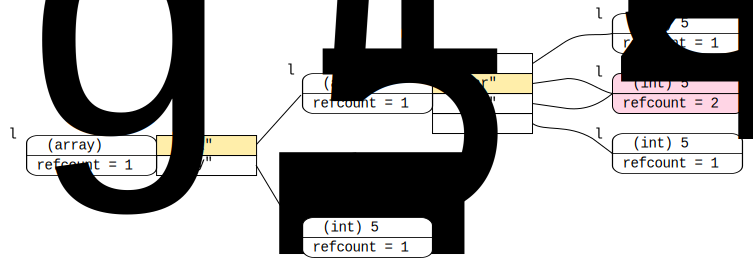
\includegraphics[scale=0.57]{diagrams/symtable.pdf}
\caption{Example heap, where the reserved location $l_g$ contains the global scope.}
\label{fig:example-heap-1}
\end{figure}

\stitle{Memory}
%
The heap, which is contained in the \kc{heap} cell, is a map $\mathbb{H} : loc \rightarrow zval$, where $loc$ is a countable set of locations $l_1, \ldots, l_n$. 
%Since zvals can contain arrays which map keys to locations containing other zvals, our memory can be seen as a graph $G = (V, E)$, where the set of vertices $V$ is the set of zvals present in the memory, and 
%$$
%E = \left \{ (v_1, v_2) \in V^2 | \texttt{Type(v1) = array} \land \exists k \in \texttt{keys(v)} | \texttt{v[k] = l} \land \mathbb{H}(l) = v_2 \right \}
%$$ 
Fig.~\ref{fig:example-heap-1} shows the heap after executing the program 
\begin{lstlisting}
$x = array("foo" => 5, "bar" => 5);
$y = 5;
next($x);
$x["baz"] = &$x["bar"];
$x[12] = 5;
\end{lstlisting}
where the elements pointed to by the array \emph{current} pointers are shaded (in yellow), and shared zvals are shaded (in red), and $l_g$ is the location containing the global scope, which is a special array where both \cc{$x} and \cc{$y} are defined. We have shown in Section~\ref{sec:deeper} how the global scope can be accessed directly via the variable \cc{$GLOBALS}.
%
In fact, just like in JavaScript, it is convenient to represent all PHP scopes as heap-allocated arrays. 



\stitle{References}
%
Several programming languages internally use references, and so does PHP, but with its own original twist. Consider running a simple program \cc{unset($y)} on the state shown in Fig.~\ref{fig:example-heap-1}. If the argument \cc{$y} were to be evaluated to a value, we would reach \cc{unset(5)} which is nonsensical. Even evaluating \cc{$y} to the location $l_5$ would not be the right choice, since in that case we could successfully free the location, but not remove the link from \cc{$y} to $l_5$ (which is stored in the array at $l_g$). This is just an example of a general class of cases, which imply that variables need to be evaluated to references of the form \kc{ref(L, K)} where \kc{L} is the address of the array or object containing the variable, and \kc{K} is the variable name. When the actual value stored in the variable is needed, further steps of reduction can be taken to  resolve the reference. 
%
This is not a trivial process, as the lookup depends on whether the reference appears on the left or right hand side of an assignment. Consider the code
\begin{lstlisting}
$x = $y;
\end{lstlisting}
where neither \cc{$x} nor \cc{$y} have been initialised. The first step is to evaluate the variables obtaining the references \kc{ref($l_g$,"x")} and \kc{ref($l_g$,"y")}. On the left-hand side, since \kc{"x"} is not an entry of the (array) scope \kc{$l_g$}, it will be created, adding a link to a fresh location. For the right-hand side, since \kc{"y"} is also not present in \kc{$l_g$}, \kc{NULL} will be returned and written to the fresh location. 

Unfortunately, since arrays are copied by value, this is not the end of the story. Consider the following program (adapted from a Zend test):\\[5pt]
%
\begin{tabular}{ll|ll}
\begin{lstlisting}
function mod_x() {
	global $x;
	$x = array('a','b');
	return 0;
}
\end{lstlisting}&&\phantom{~~}&
\begin{lstlisting}
$x = array(1, 2);
$x[0] = mod_x();
var_dump($x); 
>array(2) { [0]=> int(0)
            [1]=> string(1) "b" }
\end{lstlisting}
\end{tabular}\\[10pt]
%
If \cc{$x[0]} was evaluated to a reference before calling \cc{mod_x} (as in JavaScript), it would become \kc{ref(L1,0)}, where \kc{L1} is obtained by resolving the reference \kc{ref(L,"x")} in the current scope \kc{L}. Hence, the assignment would affect the original array and the output would still show \cc{"a"} (instead of \kc{0}) at position 0.
%
In order to model the observed PHP behaviour, we introduce a more general type of reference (\kc{lref}) which can be thought as a ``path''. In the example above, the expression \cc{$x[0]} effectively evaluates to \kc{lref(ref(L,"x"),0)}, a value which 
represent a path starting at the current scope \kc{L} and ending at the desired location. 

The \kc{lref} mechanism is also fundamental to handle assignments to arrays and objects created on-the-fly. Assume that variable \cc{$y} is undefined. Consider:
\begin{lstlisting}
$y[] -> x = 42;
\end{lstlisting}
This is indeed valid PHP code, that creates an array and an object on the fly, adds the object as element \cc{0} to the array, and adds \cc{42} as field \cc{x} to the object.

%This 
%In our framework the expression \texttt{\$x -> y[0] = "Hello!";} evaluates to 
%the (semantic) value \texttt{lref(lref(ref($l_g$, \$x), y, obj), 0, scalar)}. This 
%value, when processed in a lhs context, will, step-by-step, construct the path 
%from the environment to a fresh location representing the variable. The third argument
%to \texttt{lref}, i.e. \texttt{obj} or \texttt{array}, tells \emph{how} to initialise 
%a variable, in case it is not found. 

\stitle{Exceptions}
%
The treatment of exceptions is based on an \kc{exceptionStack} cell where we push the catch branch and the program continuation. If an exception is thrown, the catch is executed, otherwise the continuation is executed.

\stitle{HTML}
%
In general, a PHP script can be an HTML document that contains several PHP tags \cc{<?} $...$ \cc{?>} (or \cc{<?PHP} $...$ \cc{?>})  delimiting regions of PHP code that are executed as part of the same script. The HTML is treated as part of the program output, in the order it is encountered. Our semantics implements this behaviour. Hence, the \texttt{hello.php} example of Section~\ref{sec:php} is equivalent to 
\begin{lstlisting}
<HTML><Body><? echo "Hello ".$_GET["name"]."!"; ?></Body></HTML>
\end{lstlisting}



\begin{figure}[t]
\includegraphics[scale=0.22]{diagrams/config.png}
\caption{Overview of the global configuration for \kphp.}
\label{fig:config}
\end{figure}



% configuration
\stitle{Configuration}
%
The global configuration of PHP, which represents the global state of the abstract machine, consists of 42 cells, and is shown in Figure~\ref{fig:config} (we hide some of the nested cells to improve readability).
%
The \kc{script} cell contains details of the script being executed, and in particular a cell \kc{k} with the actual program in the meta-variable $\${}\mathit{PGM}$. \sm{LONG: we should mention hoisting somewhere in the paper}
%Some auxiliary cells (not shown) contain declarations hoisted in an initial parsing phase. This is necessary because a function defined at the end of a PHP script can be called by code appearing at the beginning of the script.\sm{daniele, is this ok?}
%
% alternative below is commented because confunsing with paragraph just after
%
%The \kc{script} cell contains details of the script being executed. The cell \kc{k} contains the actual program in the meta-variable $\${}\mathit{PGM}$. Some auxiliary cells (not shown) contain declarations hoisted in an initial parsing phase. This is necessary because a function defined at the end of a PHP script can be called by code appearing at the beginning of the script.\sm{daniele, is this ok?}
%
%function or class can be referenced \emph{before} its declaration, we perform a preprocessing step before running the program that essentially consists in traversing the whole AST $\mathcal{A}$ and splitting it into two parts: one containing only function and class declarations, $\mathcal{A}_d$ and the other one containing other statements, $\mathcal{A}_s$. Once the process is finished, the item $\mathcal{A}_d \kra \mathcal{A}_s$ is placed into the \texttt{k} cell, with the effect of executing all the declarations before any statement.
%
The \kc{tables} cell contains function, class and constant definitions.
%
The \kc{scopes} cell contains pointers to the various (global, super-global, current) scopes in the heap.
%
The \kc{control} cell contains the function stack, and information about the current object and class. 
%
The \kc{IO} cell contains the input and output buffers, which \K\ automatically connects to \kc{stdin} and \kc{stdout}.
%
The \kc{instrumentation} cell gathers meta-information for analysis purpose, such as the trace of semantic rules used during an execution.
%
Finally, the \kc{gc} cell is used for bookkeeping by our implementation of garbage collection.


\stitle{Semantic rules}
%
Each non-trivial language construct is described by several rewrite 
rules, each performing a step towards the full evaluation of the 
construct. Conceptually, the evaluation process happens in three steps.
%
First, \emph{structural} and \emph{context} rules are applied. Their role is to rearrange the current program so that other rules can be applied. These include for example \emph{heating} and \emph{cooling} rules, which move the arguments of an expression to the top of the computation stack (cell \kc{k}) and plug the results back once evaluated, and \emph{desugaring} rules.
%
Next, \emph{intermediate} rules apply. Their role is mostly to pre-process arguments. For example, they convert types, 
resolve	references, or read from memory.
%
%	locations. Intermediate rules are by their very nature non-reversible (e.g. after
%	the content of a location \texttt{l} is read, and it happens to be \texttt{5}, it 
%	is not possible to determine \texttt{l} again) but for most applications (see
%	section xyz) we may want to consider them non-observable, similarly to 
%	structural rules.
%	
Finally, \emph{step} rules apply. They give semantics to the actual language constructs, and cause the term being evaluated to be consumed, returning a value where necessary, so that the computation may progress.	

Besides rewrite rules, \K\ definitions also include \emph{functions}, which do not have side effects on the configuration. In our semantics, we mostly use these functions to define logical predicates for the side-conditions of other rewrite rules.

\begin{figure}[t]
(A)\quad \kc{CONTEXT ~ 'Assign(\HOLE,\_)}\\[5pt]
(B)\quad \kc{CONTEXT ~ 'Assign(\_:KResult,\HOLE)}\\[5pt]
(C)\quad $\kc{'Assign}
\left(
	\frac{\kc{R:Ref}}{\kc{convertToLoc(R)}}, \_
\right) ~~~ \kc{[intermediate]}$\\[5pt]
(D)\quad $\frac
	{\kc{'Assign(L:Loc, V:Value)}}
	{\kc{copyValueToLoc(V, L)} \kra \kc{V}}
~~~�\kc{[step]}$\\[5pt]
(E)\quad $\kc{'Assign}
\left(
	\_:\kc{KResult},
	\frac
		{\kc{V:ConvertibleToLoc}}
		{\kc{convertToLoc(V,r)}}
\right)\\[3pt] 
\phantom{(E)\quad~~}\kc{when $\neg$ isLiteral(V)}
 ~~~~~\kc{[intermediate]}$\\[5pt]
(F)\quad $\frac
	{\kc{'Assign(L:Loc,L1:Loc)}}
	{\kc{reset(L) $\kra$ 'Assign(L, L1)}}\\[3pt] 
\phantom{(F)\quad~~}\kc{when currentOverflow(L1)}
~~~~~ \kc{[intermediate]}$\\[5pt]
(G)\quad$\frac
	{\kc{'Assign(L,L1)}}
	{\kc{'Assign(L, convertToLanguageValue(L1))}}\\[3pt] 
\phantom{(G)\quad~~}\kc{when $\neg$ currentOverflow(L1)}
  ~~~~~\kc{[intermediate]}$
  
\caption{Semantic rules for assignment.}
\label{fig:assign}
\end{figure}



% semantic rules
\subsection{\kphp: Selected Semantic Rules}\label{sec:semrules}

Overall, the semantics comprises over 1,200 definitions: more than 700 are proper transition rules, the others are auxiliary definitions. 
As representative examples, we describe below the rules for assignment and functions.

\stitle{Assignment}
%
The rules for assignment are reported in Figure~\ref{fig:assign}.
Assignment is a binary expression whose arguments are evaluated left-to-right. We model this by two \kc{CONTEXT} rules that enforce that evaluation order: rule (A) does not prescribe a type for the wildcard \kc{\_} variable, that can match any term, including an unevaluated expression, whereas rule (B) can apply only after the first argument is evaluated to a \kc{KResult}. 
%
In an assignment, the LHS will evaluate to a reference. Rule (C) resolves the reference to a location.
%
If the RHS is a value, rule (D) puts the internal operation \kc{copyValueToLoc} at the front of the \kc{k} cell, and puts the value \kc{V} to be returned as a continuation. \kc{copyValueToLoc} takes care of writing \kc{V} in \kc{L}, operating recursively if \kc{V} is an array. 
%
If the RHS is not a value, then rule (E) forces it to be converted to a location.
%
If the location \kc{L1} thus obtained contains an array whose current pointer is overflown, the current pointer of the assignment target \kc{L} is reset by rule (F).
%
In the remaining cases, rule (G) converts the location \kc{L1} to a value, enabling rule (D).




\stitle{Functions}
% Function declaration
%
When a function definition is executed, we create a new entry in the \kc{functions} cell mapping the function name to a 4-tuple \kc{f(FP,FB,RT,LS)} containing the function parameter list \kc{FP}, its body \kc{FB}, its return type \kc{RT} (by value/by reference) and a pointer \kc{LS} to a scope holding the static variables (which persist across function invocations).

% Function call
%
A function call is parsed in the AST as \kc{'FunctionCall(E,Args)}. Expression \kc{E} is evaluated to a string \kc{FN} (the function name), used to retrieve from the \kc{functions} cell the various parameters described above. Execution continues by placing at the front of the \kc{k} cell the internal \kc{runFunction} term shown in the rule below, which replaces the contents of the cell \kc{k} with a new list of internal commands (the current program continuation \kc{K} will be saved on the stack).\\[7pt]
%
$\left\langle
\frac
	{\kc{runFunction(FN:String, f(FP:K, FB:K, RT:RetType, LS:Loc), Args:K)} \kra \kc{K}}
	{\left(\begin{aligned}
			\kc{processFunArgs(FP, Args)} \kra \\
			\kc{pushStackFrame(FN, K, L, CurrentClass, CurrentObj, RT, D)} \kra \\
			\kc{ArrayCreateEmpty(L1)} \kra  
			\kc{setCrntScope(L1)} \kra 
			\kc{incRefCount(L1)} \kra \\
			\kc{copyFunArgs} \kra 
			\kc{FB} \kra 
	 		\kc{'Return(NULL)}
	\end{aligned}\right)
	}\right\rangle{\kc{k}}$\\[5pt]
$\langle 
\kc{L:Loc}
\rangle_{\kc{currentScope}}\qquad
\langle 
\kc{CurrentClass:Id}
\rangle_{\kc{class}}
\qquad
\langle 
\kc{CurrentObj:Loc}
\rangle_{\kc{object}}$\\[5pt]
$\langle 
\frac{\kc{D:K}}{\kc{.}}
\rangle_{\kc{functionArgumentDeclaration}}$\\[5pt]
\kc{when fresh(L1)} ~~~~ \kc{[internal]}\\[7pt]
%
%\begin{verbatim}
%rule [run-function]:	
%	<k> runFunction(FN:String, f(FP:K, FB:K, RT:RetType, LS:Loc), Args:K) ~> K:K =>
%			processFunArgs(FP, Args) ~> 
%			pushStackFrame(FN, K, L, CurrentClass, CurrentObj, RT, D) ~> 
%			ArrayCreateEmpty(L1) ~>
%			setCrntScope(L1) ~>
%			incRefCount(L1) ~> 
%			copyFunArgs ~> 
%			FB ~> 'Return(NULL) </k>
%	<functionArgumentsDeclaration> D:K => . </functionArgumentsDeclaration>
%	<currentScope> L:Loc </currentScope>
%	<class> CurrentClass:K </class>
%	<object> CurrentObj:K </object>
%	when fresh(L1:Loc)
%	[internal]
%\end{verbatim}
%
The first command evaluates the function arguments \kc{Args} in the current scope. This depends on the declaration of the formal parameters \kc{FP}: if a parameter is declared by reference, the evaluation must stop at a location, and not fetch the value from memory. The next command pushes the current state on the stack, including the current scope \kc{L} and continuation \kc{K}. The next three commands create the function local scope \kc{L1} (the side condition \kc{fresh(L1:Loc)} means that location \kc{L1} is newly allocated), set it as the current execution scope, and increment its reference counter. The next command assigns the evaluated arguments to the formal parameters allocated on \kc{L1}. 
Finally, the function code \kc{FB} is run, followed by a default \cc{return} instruction. 








%used in the is performed in two steps: first we check wether the function being called exist; is this is the case, the function body together with the list of arguments is passed to the generic auxiliary construct \texttt{\#runFunction}, which is designed to be used for both functions and methods.

%\krule{
%\kprefix{k}{\reduce{'FunctionCall(\variable[String]{FName}\kcomma'ListWrap(\variable[KList]{Args}))}{{}\terminal{\#runFunction}({\variable[K]{FunDef}},{'ListWrap(\variable[KList]{Args})},{\dotCt{K}},{\dotCt{K}})}}
%\mathrel{}\kmiddle{functions}{\variable[String]{FName}\mapsto\variable[K]{FunDef}}
%}{isKResult(\variable[KList]{Args})}{}{}

%The \texttt{\#runFunction} operation takes four arguments: a function, a list of arguments, a class name and the location of the object. The last two arguments are optional and, as seen in the previous rule, can be skipped by passing the empty computation \texttt{.K}. 
%It has the global effect of preparing the new scope for the function, updating the current context as needed, and finally running the function.


% Discuss return

\SM{more rules? object member, method call}




\subsection{The \kphp\ Interpreter}
%
Our semantics is defined in 29 ``\texttt{.k}'' files, and consists of approximately 8500 lines of code. Compiling the semantics with the \texttt{kompile} utility of the \K\ distribution creates a directory of files for the Maude tool. We provide a Unix shell script called \texttt{kphp} that, given the name of a PHP file, invokes the \texttt{krun} utility with appropriate parameters (for the external parser, options, etc.). This runs our semantics as if it was the standard PHP interpreter.

\sm{commented out interpreter description because now there is official artefact}








% -------------------------------
% --- TEST---
% -------------------------------



\section{Testing and Validation}\label{sec:testing}
%
\sm{or ``Testing and Coverage" or ``Towards regression tests for PHP"}

In this Section we discuss the testing and validation of our (executable) semantics of PHP. Since \kphp\ is actively developed, the numbers below refer to the release current at the time of publication of this paper.


\iflong
\subsection{Test-driven semantics development}
\else\stitle{Test-driven semantics development} \fi
%
As discussed in Section~\ref{sec:intro}, there is no official document providing a specification of PHP.
%
Hence, the development of our semantics was largely test-driven.
%
The choice of specifying the semantics in \K\ meant that at each stage of this work we had a working interpreter corresponding to the fragment of PHP we specified up to that point.
This made it possible to test critical semantics rules as they were being developed.
For this ongoing testing we wrote snippets of PHP, and compared the results from our interpreter with the ones from the Zend Engine, which is the \emph{de facto} reference interpreter.

% Paragraph below is nice but too long, i ended up rewriting.
%
%Since there is no official specification for PHP which we could use as a reference (like e.g. for JavaScript), the only way we have to gain confidence in our model is testing. Thanks to the fact that our semantics is executable the process is made easier and more streamlined compared with more conventional approaches which consists in defining a semantics in a theorem prover, defining an interpreter and proving its correctness w.r.t. the semantics and finally testing it; in our case, adding or changing a new semantic rule immediately and automatically provides an updated interpreter, which can be immediately tested. Depending on the test results, we can either chose to consider the fix good and move on adding new features, or refining the rules. 

\iflong\subsection{Validation}\else
\stitle{Validation} \fi
%
As common in other PHP projects (e.g. Facebook's HHVM), we validated our semantics/interpreter by testing it against the official test suite distributed with the Zend engine. Although our semantics covers most of the core PHP language (including its challenging features, such as arrays, objects, references, aliasing, exceptions, etc.), the test suite includes many tests that refer to constructs or library functions that we do not yet support. 
%
The Zend test suite is already split into folders containing different categories of tests. We tested the semantics against all the tests in the folders \texttt{lang} (core language) and \texttt{functions}: we did not pick tests manually to avoid introducing bias. 

%
%formalization of some remaining features is still ongoing work, and However, since this is still a work in progress and, as in virtually all related work, it's nearly impossible to cover all the language and in particular the builtin/library functions, we chose to concentrate, for now, on a subset of such test suite, covering the language itself (including all of the challenging features including arrays, objects, references, exceptions etc.) and ignoring the use of library functions; this was an easy choice, since the Zend test suite is already splitter into folders containing different categories of tests including a "core language" folder, so we didn't have to pick tests manually and make (possibly biased) choices. 

The \texttt{lang} folder contains 216 tests and we pass 97 of them, the \texttt{functions} folder contains 14 and we pass 4. If a test fails, it is for one of four reasons: (i) our semantics models a feature incorrectly; (ii) a language construct is not supported by our semantics; (iii) the external parser has a bug, and returns the wrong AST; (iv) the external parser does not support some features added to PHP after version 5.0. For each failed test, our test harness shows one of these four categories. Successful tests are partitioned in 2 sets: 71 are automatically recognised as success, 26 are considered successful after manual review of the output (for example, our warning and error messages do not contain source code line numbers, because they are not recorded by the external parser).
%
\sm{LONG: spiegare i 7 failed dovuti a float che soo  considerati pass}

The only test that fails in category (i) is \texttt{031.phpt}, which tests for the erratic behaviour of \cc{current} described in Section~\ref{sec:deeper}. This fail is intentional, as we consider such behaviour to be a bug in the Zend Engine. All the other failed tests belong to categories (ii)-(iv), hence are either not supported by the semantics or by the parser. 
%
The total number of passed tests may not seem very high (JSCert passes almost 2,000 tests), but this is due to the size of the Zend test suite, and is outside our control. Moreover, many tests are non trivial, focussing on complex evaluation strategies, classes, constructors, interaction between global variables, functions, objects and aliasing. 
%
We are satisfied by this validation experiment - so far, our semantics behaves as the official PHP implementation.


%Some of those tests still contains features that we don't support yet (e.g. exceptions, advanced O.O. features), some of those uses parsing construct recently introduced in the latest versions of PHP that we don't support (e.g. square bracket array syntax), while the others pass. Hence we don't pass all of the 108 tests because many of them use features that we don't support yet. We pass, in total 48 tests. We believe this is actually an encouraging result: we passed \emph{all} the test cases which are written in the subset of the language we support. Many of them are non trivial, testing complex evaluation strategies, classes, constructors, interaction between global variables, functions, objects and so on. 

\sm{current fails are due to parser and escape characters, $\_\_$get. non-supported are detected automatically}

\begin{figure}[t]
\begin{center}
\begin{tikzpicture}
\begin{axis}[height = 5cm, width = 1.0\columnwidth, ymode=log, ymin=0,ymax=27741,enlargelimits=false]
%ymode=log
\addplot
	[const plot,fill=cyan,draw=black] 
coordinates
{
(0,27741)(1,21367)(2,19468)(3,19411)(4,18615)(5,15166)(6,11889)(7,9669)(8,8622)(9,8525)(10,8338)(11,7083)(12,6955)(13,6858)(14,6856)(15,6853)(16,6782)(17,6782)(18,5622)(19,5464)(20,5464)(21,4673)(22,4216)(23,3967)(24,3967)(25,3967)(26,3948)(27,3921)(28,3760)(29,3741)(30,3734)(31,3703)(32,3655)(33,3655)(34,3623)(35,3579)(36,3517)(37,3369)(38,3295)(39,3228)(40,3189)(41,3189)(42,3183)(43,3144)(44,2874)(45,2871)(46,2859)(47,2798)(48,2754)(49,2598)(50,2281)(51,2177)(52,1931)(53,1931)(54,1856)(55,1839)(56,1839)(57,1839)(58,1830)(59,1816)(60,1816)(61,1816)(62,1689)(63,1609)(64,1589)(65,1457)(66,1265)(67,1196)(68,1170)(69,1043)(70,1020)(71,942)(72,927)(73,863)(74,726)(75,725)(76,699)(77,668)(78,630)(79,627)(80,613)(81,612)(82,612)(83,612)(84,538)(85,531)(86,531)(87,529)(88,521)(89,444)(90,406)(91,406)(92,405)(93,405)(94,402)(95,395)(96,389)(97,365)(98,350)(99,348)(100,339)(101,336)(102,336)(103,334)(104,333)(105,312)(106,295)(107,293)(108,289)(109,288)(110,275)(111,274)(112,263)(113,256)(114,234)(115,229)(116,228)(117,227)(118,225)(119,223)(120,223)(121,223)(122,215)(123,208)(124,208)(125,208)(126,207)(127,177)(128,171)(129,171)(130,171)(131,171)(132,171)(133,171)(134,171)(135,171)(136,171)(137,171)(138,171)(139,170)(140,167)(141,163)(142,154)(143,154)(144,149)(145,138)(146,135)(147,126)(148,125)(149,121)(150,116)(151,108)(152,107)(153,107)(154,106)(155,105)(156,104)(157,101)(158,100)(159,94)(160,94)(161,93)(162,90)(163,90)(164,90)(165,89)(166,89)(167,88)(168,86)(169,86)(170,84)(171,84)(172,84)(173,83)(174,83)(175,82)(176,82)(177,79)(178,79)(179,77)(180,75)(181,75)(182,74)(183,74)(184,73)(185,73)(186,73)(187,73)(188,71)(189,67)(190,65)(191,65)(192,65)(193,62)(194,57)(195,55)(196,55)(197,54)(198,54)(199,54)(200,52)(201,51)(202,51)(203,49)(204,49)(205,49)(206,41)(207,41)(208,40)(209,39)(210,38)(211,35)(212,34)(213,34)(214,34)(215,34)(216,33)(217,31)(218,30)(219,28)(220,28)(221,28)(222,27)(223,26)(224,26)(225,25)(226,24)(227,24)(228,24)(229,24)(230,24)(231,24)(232,23)(233,22)(234,22)(235,20)(236,20)(237,20)(238,16)(239,16)(240,16)(241,16)(242,16)(243,15)(244,14)(245,14)(246,13)(247,12)(248,12)(249,12)(250,12)(251,12)(252,11)(253,11)(254,11)(255,11)(256,11)(257,11)(258,10)(259,10)(260,10)(261,10)(262,10)(263,10)(264,10)(265,9)(266,9)(267,9)(268,9)(269,9)(270,8)(271,8)(272,8)(273,8)(274,8)(275,8)(276,8)(277,8)(278,8)(279,8)(280,8)(281,8)(282,8)(283,8)(284,7)(285,7)(286,7)(287,7)(288,7)(289,7)(290,7)(291,6)(292,6)(293,6)(294,6)(295,6)(296,6)(297,6)(298,6)(299,6)(300,6)(301,6)(302,6)(303,6)(304,6)(305,5)(306,5)(307,5)(308,5)(309,5)(310,5)(311,5)(312,5)(313,5)(314,5)(315,5)(316,5)(317,5)(318,5)(319,5)(320,5)(321,5)(322,5)(323,4)(324,4)(325,4)(326,4)(327,4)(328,3)(329,3)(330,3)(331,3)(332,3)(333,3)(334,3)(335,3)(336,3)(337,3)(338,3)(339,3)(340,3)(341,3)(342,3)(343,3)(344,3)(345,3)(346,3)(347,3)(348,3)(349,3)(350,2)(351,2)(352,2)(353,2)(354,2)(355,2)(356,2)(357,2)(358,2)(359,2)(360,2)(361,2)(362,2)(363,2)(364,1)(365,1)(366,1)(367,1)(368,1)(369,1)(370,1)(371,1)(372,1)(373,1)(374,1)(375,1)(376,1)(377,1)(378,1)(379,1)(380,1)(381,1)(382,1)(383,1)(384,1)(385,1)(386,1)(387,1)(388,1)(389,1)(390,1)(391,1)(392,1)(393,1)(394,1)(395,1)(396,1)(397,1)(398,1)(399,1)(400,1)(401,1)(402,1)
} 
\closedcycle;
\end{axis}
\end{tikzpicture}
\caption{Coverage of \kphp~rules by the Zend test suite (logarithmic scale).}
\label{fig:coverage}
\end{center}
\end{figure}

\iflong \subsection{Coverage}
\else\stitle{Coverage} \fi
%
In order to assess the level of coverage of our semantics achieved by the Zend test suite, we added a \kc{trace} cell to the \kphp\ configuration, where we add the name of each rule as it is executed. Out of 721 semantics rules, 403 are executed at least once, and 318 are never executed. In Figure~\ref{fig:coverage} we show the histogram, ordered by frequency, of the executed rules. There is a big difference 
in the number of times different rules are exercised by the test suite. This is partly 
explained by our design. The small group of rules which is called more than 
$25,000$ times by the test suite corresponds to the low-level, internal rules which 
are used as building blocks by other, higher level rules. 
Internal rules that perform type conversions, such as \cc{*toInt}, are also 
intensively exercised, as expected. 
$158$ of $403$ rules are called at least $100$ times, and $264$ are called more than 
$10$ times.
Using the Zend tests alone, coverage amounts to 56$\%$ of the semantic rules. In order to achieve full-coverage, we have written targeted additional tests that cover the rules not exercised by the Zend suite.










% -------------------------------
% --- APPLICATIONS
% -------------------------------



\section{Applications}\label{sec:applications}
%
One of the main goals of our semantics is to provide a formal 
model of PHP on which semantics-based verification tools (such as abstract interpreters, type systems and
taint-checkers) can be built. Developing such tools goes beyond the scope of this paper. 
%
However, we are able to begin demonstrating the practical relevance of our semantics by showing potential applications based on the \K-Maude tool chain. In particular, the \K framework exposes Maude's explicit-state LTL model checking to the semantics~\cite{Ellison2012}, and supports symbolic execution for any language definition~\cite{Arusoaie2012b}

In this Section, we show how we used LTL model checking in conjunction with symbolic 
execution to obtain a PHP code analyser, and we analyse properties of two 3rd-party PHP functions of practical relevance.


\iflong\subsection{Model checking and symbolic execution in \K}\else
%
\subsection{Temporal Verification of PHP Programs}
\stitle{Model checking and symbolic execution in \K} \fi
%
A \K definition is eventually translated to a Maude 
rewrite theory, which can be model checked against LTL formulas 
using Maude's built-in model checker. In order to use the model checker in a meaningful way with respect to PHP, we need to instrument the semantics in two ways. First, we must decide what semantics rules should be considered as \emph{state transitions} by the model checker, tag such rules, and pass the tags to the \texttt{ --transition} compilation option. Second, we need to extend LTL with a set of atomic propositions that can be used to express interesting properties of PHP programs.

Symbolic execution has been recently introduced in \K \cite{Arusoaie2012b} and is
enabled by using the option \texttt{--backend symbolic} when compiling the \K 
definition. When symbolic mode is enabled, programs can be (optionally) 
given symbolic inputs of any of the types natively supported by the \K tool (\kc{int},\kc{float},\kc{string},\kc{bool}). 


\iflong\subsection{Temporal Verification of PHP Programs}\fi

We now describe the \kphp\ extensions needed for model checking and symbolic execution.

\stitle{State transitions}
%
\sm{beware of potential repetition with intro semantics}
%
Our semantics comprises many internal and intermediate rules, 
and it is not obvious \emph{what} exactly should represent a change in the program state 
and what should instead be considered non-observable.
Instead of fixing this notion once and for all, we allow ourselves maximum 
flexibility by defining several sets of semantic rules, and assigning a tag to each set:
\begin{itemize}
	\item \kc{step}: rules which correspond to the execution of language constructs.
	%, and are always meant to constitute a transition.
	\item \kc{internal}: rules used for operations which are not part of the user language, such as incrementing the reference counter. % These may or may not be considered as transitions depending on the granularity of the analyis.
	\item \kc{intermediate}: rules which perform auxiliary work, such as performing a type conversion on an argument before a \kc{step} or \kc{internal} rule can be applied. 
	% These normally are not considered state transitions.
	\item \kc{mem}: low-level rules which directly write the memory. 
	\item \kc{error}: orthogonal set of rules which cause a transition to an error state. 
	% This tag is typically used alongside \texttt{step}. 
\end{itemize}
%
Using these tags, we are able to reason about programs at different degrees 
of abstraction. In the rest of this section, we consider only the state transitions generated by selecting the \kc{step} rules.
An alternative would be for example to consider only the \kc{mem} rules, if the observations of interest are just the memory updates.

\stitle{A temporal logic for PHP}
%
We now define an extension of LTL with predicates over \kphp\ configurations (i.e. PHP program states).
%
Given a PHP program, we would like to be able to express conditions such as: ``variable \cc{$usr} never contains \cc{'admin'}'', or ``the local variable \cc{$y} of function \cc{foo} will at some point be aliased to the global variable \cc{$y}".  Moreover, we also want to be able to reason about \emph{correspondence assertions}~\cite{Woo1993}, by labelling program
points and stating properties such as ``after reaching label \cc{'login'} variable \cc{$sec} always contains 
\cc{1}''.
%
To this end, we introduce predicates such as \kc{eqTo} (equals to), \kc{gv} (global variable), \kc{fv} (function variable).
The LTL formulas corresponding to the informal specifications above are,
respectively:\\[7pt]
%
\phantom{doh}$\square \neg $\kc{eqTo(gv(var('usr')),val('admin'))}\\[4pt]
\phantom{doh}$\Diamond $\kc{alias(fv('foo',var('y')),gv(var('y')))}\\[4pt]
\phantom{doh}\kc{label('login')}$ \Rightarrow  \square $\kc{eqTo(gv(var(sec)),val(1))}\\[7pt]
%
Moreover, we also found useful to be able to reason about types. For example, the 
following formula says that variable \cc{$y} always has type \cc{integer} during
the execution of function \cc{foo}:\\[7pt]
%
\phantom{doh}$\Box $(\kc{inFun('foo')}$\Rightarrow$\kc{has\_type(fv('foo',var('y')),integer)})\\[7pt]
%
%\stitle{Predicate semantics}
%
Each new predicate should be given a precise meaning in the context of the \kphp\ configuration.
We illustrate how we do that through the example of predicate \kc{eqTo(e1,e2)}. 
Given a configuration \kc{B}, we need to define when it satisfies the predicate:\\[7pt]
%
\phantom{doh}$\kc{B} \models \kc{eqTo(e1,e2)} \Leftrightarrow \kc{eval(B,e1) = eval(B,e2)}$\\[7pt]
%
meaning, that formula \kc{eqTo(e1,e2)} is true 
for \kc{B} if and only if \kc{e1} and \kc{e2} evaluate to the same value.
%
The definition of functions such as \kc{eval} is crucial, as it connects the semantics to the model checker.
%
These functions should be written in purely functional style and avoid side effects. In practice they are pretty simple, as they only need to inspect a configuration using pattern matching.
%
As another example, consider predicate \kc{alias(e1,e2)}:\\[7pt]
%
\phantom{doh}$\kc{B} \models \kc{alias(e1,e2)} \Leftrightarrow \kc{lvalue(B,e1) = lvalue(B,e2)}$\\[7pt]
%
Function \kc{lvalue} returns the location of the heap where its argument is stored, so the predicate is true when the arguments are aliased or identical.
%
We use similar techniques to give semantics to all of our predicates, which can be used to form extended LTL formulas together with standard LTL connectives.

\stitle{Limitations}
%
The approach described here suffers from the known limitations of the underlying verification techniques.
In particular, explicit state LTL model checking will struggle to handle programs that generate large state spaces that depend heavily on the program inputs. The support for symbolic execution mitigates this problem, but as common to this approach it does not handle higher order data structures, such as objects, and struggles with loops depending on symbolic values.
%
Despite these limitations, in the rest of this section we show that we can indeed verify some non-trivial properties of real PHP code.







\subsection{Case Study: Input Validation}
%
In our first example of model checking, we consider the function
\cc{PMA_isValid} taken from the source code of \texttt{phpMyAdmin}~\cite{phpMyAdminWeb}, one of the most common open source web applications, which provides a web interface to administer an SQL server.

\cc{PMA_isValid} takes three arguments (\cc{&$var}, \cc{$type},	and \cc{$compare}) and returns a boolean.
Its purpose is to  
 ``validate'' the argument \cc{$var} according to different criteria that depend on the other two 
arguments. We analyse the full source code of \cc{PMA_isValid}, which is shown in Appendix\iflong~\ref{sec:PMA}.\else~A.1 of the extended version of this paper, available on \website.\fi

In the simplest case, \cc{PMA_isValid} simply checks that \cc{$var} is of the same 
type (or meta type) specified by \cc{$type}, ignoring the remaining argument \cc{$compare}: 
\begin{lstlisting}
PMA_isValid(0, "int"); 			// true
PMA_isValid("hello", "scalar"); 	// true
PMA_isValid("hello", "numeric"); 	// false
PMA_isValid("123", "numeric");		// true 
PMA_isValid("anything", false); 	// always true 
\end{lstlisting}
A more interesting case is when the argument \cc{$type} is instantiated with one of \cc{"identical"}, \cc{"equal"} or \cc{"similar"}. 
In such case, the validation of \cc{$var} is performed against \cc{$comparison}, according to the 
criterion specified by \cc{$type}:
\begin{lstlisting}
PMA_isValid(0, "identical", 1);		// false
PMA_isValid(0, "equal", 1);		// true
PMA_isValid("hello", "similar", 1);	// false
\end{lstlisting}
If \cc{$type} is an array, validation succeeds if \cc{$var} is an element of that array. 
If \cc{$type} is \cc{"length"}, validation succeeds if \cc{$var} is a scalar with a string length greater that zero,
If \cc{$type = false}, validation always succeeds. 
\begin{lstlisting}
PMA_isValid(0, array(0,1,2)); 	// true
PMA_isValid(true, "length");	// true, as (string) true = "1"
PMA_isValid(false, "length"); 	// false, as (string) false = ""
\end{lstlisting}
%Hence, \cc{PMA_isValid} is a ``swiss knife'' function used to actually compare
%variable values, or their type, or to check wether they have a positive string 
%length or belong to a given array, where the intended behaviour/execution path is 
%selected as a result of a combination of the values and types of the three arguments. 
The developer had an informal specification of this function in mind, which he wrote
in a comment at the beginning of the function. However, it is not obvious wether such 
specification is met by the actual implementation.
Leveraging model checking and symbolic execution we are able to prove that the 
function behaves as expected, by verifying each sub-case.

We first write some code accepting (possibly) symbolic inputs, and calling the function:
\begin{lstlisting}
$var = user_input();		// symbolic 
$type = user_input();		// symbolic
$compare = user_input();	// symbolic
$result = PMA_isValid($var, $type, $compare);
\end{lstlisting}
then we attempt to verify multiple times the LTL formula
$$
\Diamond \kc{eqTo(gv(var('result'),val(true)))}
$$ 
each time providing different combinations of symbolic and concrete inputs, until all of the cases discussed above are covered.
Indeed, these verifications succeed, proving the correctness of the function. 

As a concrete example, in order to prove that the result of calling \cc{PMA_isValid} with \cc{$type="numeric"} is \cc{true} when \cc{$var} is an \cc{integer}, we provide the symbolic input \cc{??symInt(x)} to \cc{$var}, and the concrete
input \cc{"numeric"} to \cc{$type}. 
%
We proved analogous results for the case of \cc{float} variables, and for the other similar cases.
%
We proved that \cc{PMA_is_Valid($var, "similar", $compare)} returns \cc{true} for any \cc{integer} \cc{$var} and \cc{string} \cc{$compare}, by  providing symbolic values \cc{??symInt(x)} and \cc{??symString(y)} to \cc{$var} and \cc{$compare}.








\subsection{Case Study: Cryptographic Key Generation}\label{sec:cs2}

In our second example, we consider the Password-Based Key Derivation Function \cc{pbkdf2} from the PHP distribution~\cite{pbkdf2Web}.
\cc{pbkdf2} takes five parameters: the name of the algorithm to be used for hashing (\cc{$algo}), 
a \cc{$password}, a \cc{$salt}, an iteration \cc{$count} and the desired 
\cc{$key_length}. It returns a key derived from \cc{$password} and \cc{$salt} whose
length is \cc{$key_length}. We wish to prove that the function always returns a 
\cc{string}, and that its length is equal to the requested \cc{$key_length}. 

Using the same approach as for the previous example, we write some initial code accepting
(possibly) symbolic inputs, and calling the function:
\begin{lstlisting}
$algo = "sha224";
$pass = user_input(); 	// symbolic input
$salt = user_input(); 	// symbolic input
$count = 1;
$key_len = 16;
$result = pbkdf2($algo, $pass, $salt, $count, $key_len);
\end{lstlisting}
Next, we run the model checker on our query formulae:
%
\begin{enumerate} 
\item The result is a string: 
$\Diamond \kc{has\_type(gv(var('result')),string)}$
%
\item The length of the output is as requested:
$$
\Diamond \kc{eqTo(gv(var('key\_len')),len(gv(var('result'))))}
$$
%
\item The length of the string stored in local variable \cc{$output} grows, and eventually becomes greater than the required output length:\\[5pt]
$\Box
\big(~(\kc{inFun('pbkdf2')} \wedge \neg\kc{inFun('top')} \wedge \Diamond \kc{inFun('top')}) 
  \implies$ \\
  \phantom{qqq}$(\Diamond (\kc{geq(len(fv('pbkdf2',var('output'))), fv('pbkdf2', var('key\_len'))})$\\ 
  \phantom{qqq}$\mathcal{U} ~\kc{inFun('top')})~\big)$

\end{enumerate}

Property (3) shows that property (2) is non-trivial.\sm{explain this better} Moreover, it illustrates a technically more intriguing LTL formula.
%
Using the model checker, we are able to verify that all three properties in less than a minute.
%
Unlike the previous example, which we were able to run and analyse out-of-the-box, in this case we had to provide implementations for an number of functions (such as \cc{hash}), which belong to libraries outside of the core language.
%
For the sake of verification, we only provide simple stubs for these functions, making sure to preserve the type and output length properties of their original versions.
%
The complete source code of \cc{pbkdf2} and related functions can be found in Appendix\iflong ~\ref{sec:pbkdf2}.\else~A.2 of the extended version of this paper, available on \website. \fi
 
 

% -------------------------------
% --- LIMITATIONS
% -------------------------------



\section{Limitations and Future Work}

A formal, executable semantics of a real programming language is too large a task to be completed in one single effort. This paper models the core of PHP, which includes the features we considered more important and instructive, leaving out some non-core features and the numerous language extensions.
%
In this Section, we summarise what we left out of the current formalisation, and indicate what we think are the next priorities to take this work further. 

\stitle{Parsing limitations} 
%
As discussed in Section~\ref{sec:testing}, the external parser we currently use does not understand some language constructs introduced after version 5.0, such as for example the literal array syntax with square brackets (\cc{[1,2,3]} instead of \cc{array(1,2,3)}). It also does not parse correctly some constructs such as \cc{$this->a[]} which gets parsed as \cc{$this->(a[])} instead of \cc{($this->a)[]}.
%
In future development, we plan to adopt a fully-compliant external parser.

%\stitle{Reliance on \K\ types}
%%
%Other issues are related to the fact that we currently rely, for some things, on \K's builtins facilities, which do not always match the exact features we would like to model. An example is the conversion from a string to an integer. Although this can be done by \K~ via builtin helper functions, the semantics of this operation in PHP can assume more complicated forms, which are not permitted by the \K~ tool. 
%In order to fix this, in future work, we will define from scratch the defined operations (instead as of using the builtin ones).


\stitle{Missing language features}
%
We have not (yet) implemented a number of non-core language features, and in particular: bit-wise operators, 
most escape characters, regular expressions, namespaces, interfaces, abstract classes, iterators, magic methods 
and closures. 
%
We do not foresee significant obstacles in integrating these into \kphp.
% 
For example, magic methods are special object methods (\cc{__toString, __get, __call}, etc.) with reflective behaviour that are called automatically by PHP. JavaScript has similar reflective methods, and techniques to formalise them are well documented~\cite{Maffeis2008,Bodin}. As a taster, we included in the core language the \cc{__construct} magic method, which is used by the \cc{new} command when creating a fresh object.
%
Since version 5.3, PHP includes anonymous functions, implemented as objects of a special \cc{Closure} class. These are not supported by our parser, but can be easily modelled in our semantics by adding to the object \kc{OID} constructor an optional argument pointing to the entry of the \kc{functions} cell where the anonymous function definition would be stored (using the same mechanism of regular functions).

\stitle{Internal functions}
%
As in related projects, a challenge when dealing with a real language is the sheer number of built-in library functions that operate on numbers, strings, arrays and objects. At the moment we model just a small, representative subset of them (e.g. \cc{strlen}, \cc{substr}, \cc{count}, \cc{is_int}, \cc{is_float}, \cc{var_dump}, etc.). Where possible, we define such functions in PHP directly; we define them in \K\ in the remaining cases (this corresponds to PHP native functions implemented in C). 

\stitle{Language extensions}
%
Language extensions, such as the functions that provide access to an SQL database, or that connect a PHP script with a server (and hence with the network) are of fundamental importance for developing web applications, but are squarely beyond the scope of our current work. Our goal is to provide a sound semantic foundation to the core language that glues all such functions together. 
%
Until (semi-)automated techniques that help giving semantics to language extensions are developed, our view is that such extensions need to be investigated on a case-by-case basis. Often, they can be abstracted in terms of approximate information such as for example their types, taint behaviour, or side effects, as exemplified by our case study of Section~\ref{sec:cs2}. 



% -------------------------------
% --- Related Work
% -------------------------------



\section{Related Work}

In this Section, we discuss related work on the mechanised formalisation of programming languages, and on the analysis of PHP.

\iflong\subsection{Mechanised formalisation of programming languages}\else
\stitle{Mechanised formalisation of programming languages} \fi
%
% Related work with theorem provers
Proof assistants such as Coq~\cite{Huet2007}, Isabelle/HOL~\cite{Nipkow2002}, are a popular choice for the mechanised specification of programming languages. 
%
For example, HOL was used by Norrish~\cite{Norrish1998}
to specify a small-step operational semantics of C, and to prove meta-properties of the
language. Blazy and Leroy, as part of the CompCert project~\cite{Blazy2009}, have built a verified compiler for a significant fragment of C, formalised in Coq. They have proved that the semantics of source programs is preserved by the compilation process.
%
In the JSCert project~\cite{Bodin}, Bodin \etal\ have built a mechanised formalisation of JavaScript (ECMAScript 5) 
and tested it again the ECMA262 test suite. In Coq, they have developed an inductive definition of the semantics and a separate fixpoint definition of a JavaScript interpreter, and proved that the interpreter is sound with respect to the semantics. From the Coq fixpoint definition they have automatically extracted OCAML code to execute the interpreter. 

%% Advantages of theorem provers
%Proof assistants are powerful in that they can 
%be used to \emph{reason} about the language as a whole (e.g. to to prove type 
%soundness or memory safety theorems), and can be used to develop \emph{certified}
%interpreters and tools.
%% Disadvantages of theorem provers
%However, there are also several disadvantages. Mastering those systems require quite
%a substantial learning curve, and definitions can easily become verbose and hard to 
%maintain. More importantly, proof assistant formalizations are not 
%directly executable, meaning that in order to execute the semantics is necessary 
%to develop an interpreter and prove its correctness w.r.t. the semantics. 

In the \K\ framework instead a semanticist may directly focus on writing and analysing language definitions: execution is taken care of by the tool.  
%
Ellison and Rosu~\cite{Ellison2012} have defined an executable formal semantics of C
in \K~\cite{Rosu2010}. Their formalisation has been
extensively tested against the GCC torture suite~\cite{gcc-test}, and they demonstrate examples of the debugging and model checking C code using the built-in capabilities of \K.
%
On a smaller scale, \K, has also been used to formalise, Python~\cite{Python-in-K}, Scheme~\cite{Meredith2007}, Verilog~\cite{Meredith2010}, Haskell~\cite{Haskell-in-K} and Java~\cite{Java-in-K}. 
%
A number of program analysis techniques such as \emph{symbolic execution}~\cite{Arusoaie2012b}, \emph{program logics}~\cite{Rosu2012} and \emph{program equivalence}~\cite{Lucanu2013} are being developed and incorporated into the \K, extending the potential benefits of defining a programming language semantics in this framework.

For PHP, we followed the approach of~\cite{Ellison2012}. In the absence of a specification document, it was crucial to be able to immediately execute operational semantics rules as they were being developed, in order to compare with the reference implementation of the language. Moreover, we were intrigued by the possibility to leverage existing model checking and symbolic execution capabilities to demonstrate our semantics at work.

The approach to define an executable semantics of a \emph{real} programming language and validating it by testing against official test suites was trail-blazed by Guha \etal~\cite{Guha2010}, who give semantics to JavaScript via a translation to a simpler intermediate language called $\lambda_{JS}$, formalised in the PLT Redex tool~\cite{Klein:2012} (which also takes care of execution).
%
More recently, the same approach was adopted by Politz \etal~\cite{Politz2013} to Python.


\iflong\subsection{PHP analysis}\else
\stitle{PHP analysis} \fi
%
Analysis of PHP and other web languages is an important topic, given the prevalence of security flaws such as XSS, CSRF and SQL injection. There are many research and commercial tools that statically analyse PHP code, including Pixy~\cite{Jovanovic2010}, WebSSARI~\cite{Xie2006}, PHP-Sat~\cite{Bouwers2007} and HP Fortify~\cite{Fortify-web}.
%
According to the respective papers, all of these tools have specific weaknesses related to language features that are hard to understand and analyse. For example, Pixy and WebSSARI do not follow taint flows across objects. We believe that the next generation of static analysis tools can benefit from a precise, formal semantics of the language.

We are the first to present such a semantics for PHP. The only previous work we are aware of that looks in depth as some aspect of PHP semantics is an analysis of the array-copying mechanism of PHP by Tozawa \etal~\cite{Tozawa2009}. They formalise a tiny fragment of the language that suffices to describe  the array copy mechanism, and show a flaw in a runtime optimisation used by the Zend engine. Their work sheds light on how complex the array semantics in PHP is, and was an inspiration for us to dig deeper into the PHP semantics.
%
%It is surprising that the formalisation of PHP has received so little attention. For example, JavaScript, which can be considered PHP's client-side counterpart, has received a lot more attention, and already has at least three different formalizations (see, e.g.~\cite{JSCert-web} ~\cite{Guha2010}).












% -------------------------------
% --- CONCLUSIONS
% -------------------------------

\section{Conclusions}

In this paper we described the first formal semantics of PHP. 
%
We focussed on the core language, leaving language extensions and library functions for future work.
%
Our semantics is executable, meaning that from the formal definition we automatically obtained a trusted interpreter of PHP, which we used for testing and debugging the semantics.

We validated the semantics by showing that is passes all the Zend tests applicable to the PHP fragment we modelled, and we achieved full coverage of our semantic rules by defining new ad-hoc tests. 
%
Given a mechanised semantics, it is still an open research problem how to automatically generate a comprehensive regression test suite for a language.
%
If such a systematic approach to test generation was available, our semantics could be the basis for a regression test suite for PHP implementations.

Leveraging built-in features of \K\ and Maude, we also provided a proof-of-concept infrastructure for the verification of PHP programs, which we demonstrated on two realistic examples.
%
Our work is a first step towards defining semantics-based, static-analysis tools that provide formal guarantees for PHP web applications.




\stitle{Acknowledgments} 
%
We are indebted to Antoine Delignat-Lavaud for many insightful discussions on the arcana of PHP. We would also like to thank the \K team for their technical support on using the \K framework, and Shijiao Yuwen for useful comments on an earlier version of the \kphp\ semantics.
%
Filaretti and Maffeis are supported by EPSRC grant EP/I004246/1.










% ===============================================================================
% === Bibliography ==============================================================
% ===============================================================================


\bibliographystyle{plain}
\bibliography{bib/kphp.bib}

\iflong

\newpage

\appendix 

\section{Source code}\label{sec:appendix}

\subsection{The function \texttt{PMA\_isValid} from phpMyAdmin}\label{sec:PMA}

\begin{lstlisting}

/**
 * checks given $var against $type or $compare
 *
 * $type can be:
 * - false       : no type checking
 * - 'scalar'    : whether type of $var is integer, float, string or boolean
 * - 'numeric'   : whether type of $var is any number repesentation
 * - 'length'    : whether type of $var is scalar with a string length > 0
 * - 'similar'   : whether type of $var is similar to type of $compare
 * - 'equal'     : whether type of $var is identical to type of $compare
 * - 'identical' : whether $var is identical to $compare, not only the type!
 * - or any other valid PHP variable type
 *
 * <code>
 * // $_REQUEST['doit'] = true;
 * PMA_isValid($_REQUEST['doit'], 'identical', 'true'); // false
 * // $_REQUEST['doit'] = 'true';
 * PMA_isValid($_REQUEST['doit'], 'identical', 'true'); // true
 * </code>
 *
 * NOTE: call-by-reference is used to not get NOTICE on undefined vars,
 * but the var is not altered inside this function, also after checking a var
 * this var exists nut is not set, example:
 * <code>
 * // $var is not set
 * isset($var); // false
 * functionCallByReference($var); // false
 * isset($var); // true
 * functionCallByReference($var); // true
 * </code>
 *
 * to avoid this we set this var to null if not isset
 *
 * @param mixed &$var    variable to check
 * @param mixed $type    var type or array of valid values to check against $var
 * @param mixed $compare var to compare with $var
 *
 * @return boolean whether valid or not
 *
 * @todo add some more var types like hex, bin, ...?
 * @see     http://php.net/gettype
 */




function PMA_isValid(&$var, $type = 'length', $compare = null)
{

    if (! isset($var)) {
        // var is not even set
        return false;
    }

    if ($type === false) {
        // no vartype requested
        return true;
    }

    if (is_array($type)) {
        return in_array($var, $type);
    }

    // allow some aliaes of var types
    $type = strtolower($type); 
    switch ($type) {
    case 'identic' :
        $type = 'identical';
        break;
    case 'len' :
        $type = 'length';
        break;
    case 'bool' :
        $type = 'boolean';
        break;
    case 'float' :
        $type = 'double';
        break;
    case 'int' :
        $type = 'integer';
        break;
    case 'null' :
        $type = 'NULL';
        break;
    }

    if ($type === 'identical') {
        return $var === $compare;
    }

    // whether we should check against given $compare
    if ($type === 'similar') {
        switch (gettype($compare)) {
        case 'string':
        case 'boolean':
            $type = 'scalar';
            break;
        case 'integer':
        case 'double':
            $type = 'numeric';
            break;
        default:
            $type = gettype($compare);
        }
    } elseif ($type === 'equal') {
        $type = gettype($compare);
    }

    // do the check
    if ($type === 'length' || $type === 'scalar') {
        $is_scalar = is_scalar($var);
        if ($is_scalar && $type === 'length') {
            return (bool) strlen($var);
        }
        return $is_scalar;
    }

    if ($type === 'numeric') {
        return is_numeric($var);
    }
    
    if (gettype($var) === $type) {
        return true;
    }

    return false;
}
\end{lstlisting}

\subsection{Case study 2: The function \texttt{pbkdf2} from \url{php.net}}\label{sec:pbkdf2}

\begin{lstlisting}

/*
 * PBKDF2 key derivation function as defined by RSA's PKCS #5: 
 * https://www.ietf.org/rfc/rfc2898.txt
 * $algorithm - The hash algorithm to use. Recommended: SHA256
 * $password - The password.
 * $salt - A salt that is unique to the password.
 * $count - Iteration count. Higher is better, but slower. 
 * Recommended: At least 1024.
 * $key_length - The length of the derived key in bytes.
 * $raw_output - If true, the key is returned in raw binary format. 
 * Hex encoded otherwise.
 * Returns: A $key_length-byte key derived from the password and salt
 * Test vectors can be found here: https://www.ietf.org/rfc/rfc6070.txt
 * This implementation of PBKDF2 was originally created by defuse.ca
 * With improvements by variations-of-shadow.com
 */

function pbkdf2($algorithm, $password, $salt, $count, 
                $key_length, $raw_output = false)
{
    $algorithm = strtolower($algorithm);
    if(!in_array($algorithm, hash_algos(), true))
        die('PBKDF2 ERROR: Invalid hash algorithm.');
    if($count <= 0 || $key_length <= 0)
        die('PBKDF2 ERROR: Invalid parameters.');

    $hash_length = strlen(hash($algorithm, "", true));
    $block_count = ceil($key_length / $hash_length);

    $output = "";
    for($i = 1; $i <= $block_count; $i++) {
        // $i encoded as 4 bytes, big endian.
        $last = $salt . pack("N", $i);
        // first iteration
        $last = $xorsum = hash_hmac($algorithm, 
        		$last, $password, true);
        // perform the other $count - 1 iterations        
        for ($j = 1; $j < $count; $j++) {
            $xorsum ^= ($last = hash_hmac($algorithm, 
            $last, $password, true));
        }
        $output .= $xorsum;
    }
    
    if($raw_output)
        return substr($output, 0, $key_length);
    else
        return bin2hex(substr($output, 0, $key_length));
}
\end{lstlisting}



\stitle{Auxiliary functions}
%
Below, we show the simplified implementation of the functions invoked by \cc{pbkdf2}.
%
\SM{add more?}



\begin{lstlisting}

// approximation of 'strtolower': returns the string unchanged
function strtolower($s) 
{
	return $s;
}

// check wether element $x is in $array
function in_array($x, $array) 
{
	foreach ($array as $elem)
	{
		if ($x == $elem)
			return true;
	}
	return false;
}

// emulates PHP hash_algos() built-in function 
function hash_algos()
{	
	$x = array(
		"md2",
		"md4",
		"md5",
		"sha1",
		"sha224",
		"sha256",
		"sha384",
		"sha512",
		"ripemd128",
		"ripemd160",
		"ripemd256",
		"ripemd320",
		"whirlpool",
		"tiger128,3",
		"tiger160,3",
		"tiger192,3",
		"tiger128,4",
		"tiger160,4",
		"tiger192,4",
		"snefru",
		"snefru256",
		"gost",
		"adler32",
		"crc32",
		"crc32b",
		"salsa10",
		"salsa20",
		"haval128,3",
		"haval160,3",
		"haval192,3",
		"haval224,3",
		"haval256,3",
		"haval128,4",
		"haval160,4",
		"haval192,4",
		"haval224,4",
		"haval256,4",
		"haval128,5",
		"haval160,5",
		"haval192,5",
		"haval224,5",
		"haval256,5");
	return $x;
}

// returns an array containing the expected output for the 
// various hashing algorithms
function hash_algos_len()
{
	$x = array(
		"md2" => 32,
		"md4" => 32,
		"md5" => 32,
		"sha1" => 40,
		"sha224" => 56,
		"sha256" => 64,
		"sha384" => 96,
		"sha512" => 128,
		"ripemd128" => 32,
		"ripemd160" => 40,
		"ripemd256" => 64,
		"ripemd320" => 80,
		"whirlpool" => 128,
		"tiger128,3" => 32,
		"tiger160,3" => 40,
		"tiger192,3" => 48,
		"tiger128,4" => 32,
		"tiger160,4" => 40,
		"tiger192,4" => 48,
		"snefru" => 64,
		"snefru256" => 64,
		"gost" => 64,
		"adler32" => 8,
		"crc32" => 8,
		"crc32b" => 8,
		"salsa10" => 128,
		"salsa20" => 128,
		"haval128,3" => 32,
		"haval160,3" => 40,
		"haval192,3" => 48,
		"haval224,3" => 56,
		"haval256,3" => 64,
		"haval128,4" => 32,
		"haval160,4" => 40,
		"haval192,4" => 48,
		"haval224,4" => 56,
		"haval256,4" => 64,
		"haval128,5" => 32,
		"haval160,5" => 40,
		"haval192,5" => 48,
		"haval224,5" => 56,
		"haval256,5" => 64);	
	return $x;
}

// simple ceiling function
function ceil ($x) 
{
	$x_int = (int) $x;
	
	if ($x === 0)
		return 0;
	if ($x == $x_int)
		return $x_int;
	else
		return $x_int + 1;
	
	return 123;
}

// approximate 'hash' function - only preserves expected output length
// and type (which is string)
function hash($algo, $pass, $raw = false)
{
	$algos_len = hash_algos_len();
	$exp_len = $algos_len[$algo];
	$out = "";
	for ($i = 0; $i < $exp_len; $i++)
	{
		$out .= "*";
	}
	return $out;
}

// approximate 'hash_hmac' function - actually uses 'hash' (see above)
function hash_hmac($algo, $salt, $pass, $raw = false)
{
	$result = hash($algo, $pass, $raw);
	return $result;
}

function bin2hex($x) {return $x;}

function pack($format, $x) {return $x;}

\end{lstlisting}
\fi

\iflong\else
% Artefact description
%% Template for one-page artifact description appendices in lncs volumes
% Written by Camil Demetrescu and Erik Ernst
% April 8, 2014

% ARTIFACT: do not change the following line
\clearpage\appendix\section{Artifact Description}

% ARTIFACT: please note that the rest of this file contains (1) LaTeX commands
% and environments that you must use in the way they are given here, and in the
% same order, each producing one section of text; (2) example data filling in
% those commands and environments with text to show how they may be used; you
% must preserve the former and replace the latter by information concerning
% your artifact; the comments describe each of these sections to indicate
% their purpose; also note that the entire appendix must fit on one page

% ARTIFACT: section on authors of the artifact; note that this may differ from
% the list of authors of the paper, e.g., you may wish to mention other people
% who contributed to the artifact, but who did not co-author the paper
\artifactauthors{Daniele Filaretti and Sergio Maffeis.}

% ARTIFACT: section giving a brief summary of the purpose of the artifact
\begin{summary}
  The provided package is designed to support repeatability of the experiments of the paper: 
  in particular, it allows users to test the \kphp{} interpreter and symbolic model checker on a variety of 
  examples, including the ones discussed in the paper. 
  We provide details on how to install and build \kphp{}, together with step-by-step instructions for running the examples and getting users started with their own experiments.
\end{summary}

% ARTIFACT: section on the contents of the artifact (code, data, etc.)
\begin{content}
  The artifact package includes:
  \begin{itemize}
  \item the complete source files;
  \item a build of the \K\ Framework (which is needed for running \kphp{});
  \item all the examples discussed in the paper;
  \item a self-contained Linux-based virtual machine which can be used to run the artifact, if a user does not want to install \kphp{} and \K\ directly;
  \item detailed instructions on how to build and use the artifact in {\tt index.html}.
  \end{itemize}
\end{content} 

% ARTIFACT: section containing links to sites (e.g., github) holding the
% latest version of the code, if any
\begin{getting}
  The artifact, endorsed by the Artifact Evaluation Committee of ECOOP'14,  is available free
  of charge as supplementary material of this paper on SpringerLink. \kphp{} is still under development. The latest version of \kphp{}, together with a user-friendly
  web interface, is available online at \url{http://www.phpsemantics.org}.
\end{getting} 

% ARTIFACT: section specifying the platforms on which the artifact is known to
% work, including requirements beyond the operating system such as large
% amounts of memory or many processor cores
\begin{platforms}
  The \K\ tool binaries (needed for running \kphp{})
  run best on Linux and OS X. On Windows, Cygwin emulation must be used, 
  which may slow down execution. 
  The self-contained Linux-based VMware virtual machine we provide
  (included in the package) can be used in case of installation problems
  on non-standard system configurations. 
\end{platforms}

% ARTIFACT: section specifying the license under which the artifact is
% made available
\license{EPL-1.0 (\url{http://www.eclipse.org/legal/epl-v10.html}).}

% ARTIFACT: section specifying the md5 sum of the artifact master file
% uploaded to SpringerLink, enabling downloaders to check that the file is the
% expected version and suffered no damage during download
\mdsum{ed21cb3680e42078bc7cd2778ecfe03f.}

% ARTIFACT: section specifying the size of the artifact master file uploaded
% to SpringerLink
\artifactsize{281.6 MB.}

% ARTIFACT: include here any additional references, if needed...

%\bibliographystyle{unsrt}
%\begin{thebibliography}{10}
%...
%\end{thebibliography}

\fi
\end{document}
